% Created 2021-05-08 Sat 19:52
% Intended LaTeX compiler: pdflatex
\documentclass{tufte-book}
\usepackage[utf8]{inputenc}
\usepackage[T1]{fontenc}
\usepackage{graphicx}
\usepackage{grffile}
\usepackage{longtable}
\usepackage{wrapfig}
\usepackage{rotating}
\usepackage[normalem]{ulem}
\usepackage{amsmath}
\usepackage{textcomp}
\usepackage{amssymb}
\usepackage{capt-of}
\usepackage{hyperref}
\hypersetup{colorlinks}% uncomment this line if you prefer colored hyperlinks (e.g., for onscreen viewing)
\usepackage{amsfonts, soul, microtype}



%toc
%\usepackage{titletoc}
%

% section and subsection headings
\usepackage{titlesec}

\titleformat{\section}
  {\normalfont\fontsize{12}{15}\bfseries}{\thesection}{1em}{}

\usepackage[linesnumbered, ruled]{algorithm2e}
\usepackage{algorithmic}
\usepackage[parfill]{parskip}

%\usepackage{thmtools}
%\theoremstyle{definition}
\newtheorem{theorem}{Theorem}[chapter]
\newtheorem{lemma}[theorem]{Lemma}
\newtheorem{corollary}[theorem]{Corollary}
\newtheorem{proposition}[theorem]{Proposition}
\newtheorem{property}[theorem]{Property}
\newtheorem{fact}[theorem]{Fact}
\newtheorem{problem}[theorem]{Problem}
\newtheorem{exercise}[theorem]{Exercise}
\newtheorem{example}[theorem]{Example}
\newtheorem{definition}[theorem]{Definition}
\newtheorem{remark}[theorem]{Remark}
\newtheorem{conjecture}[theorem]{Conjecture}
\newtheorem{claim}[theorem]{Claim}

%Book metadata
%\title{A Tufte-Style Book\thanks{Thanks to Edward R.~Tufte for his inspiration.}}
%\author[The Tufte-LaTeX Developers]{The Tufte-LaTeX\ Developers}
%\publisher{Publisher of This Book}

%%
% If they're installed, use Bergamo and Chantilly from www.fontsite.com.
% They're clones of Bembo and Gill Sans, respectively.
%\IfFileExists{bergamo.sty}{\usepackage[osf]{bergamo}}{}% Bembo
%\IfFileExists{chantill.sty}{\usepackage{chantill}}{}% Gill Sans

%\usepackage{microtype}
\usepackage{hyperref}
%%
% Just some sample text

%%
% For nicely typeset tabular material
\usepackage{booktabs}

%%
% For graphics / images
\usepackage{graphicx}
\setkeys{Gin}{width=\linewidth,totalheight=\textheight,keepaspectratio}
\graphicspath{{graphics/}}

% The fancyvrb package lets us customize the formatting of verbatim
% environments.  We use a slightly smaller font.
\usepackage{fancyvrb}
\fvset{fontsize=\normalsize}

%%
% Prints argument within hanging parentheses (i.e., parentheses that take
% up no horizontal space).  Useful in tabular environments.
%\newcommand{\hangp}[1]{\makebox[0pt][r]{(}#1\makebox[0pt][l]{)}}

%%
% Prints an asterisk that takes up no horizontal space.
% Useful in tabular environments.
%\newcommand{\hangstar}{\makebox[0pt][l]{*}}

%%
% Prints a trailing space in a smart way.
\usepackage{xspace}


% Prints the month name (e.g., January) and the year (e.g., 2008)
\newcommand{\monthyear}{%
  \ifcase\month\or January\or February\or March\or April\or May\or June\or
  July\or August\or September\or October\or November\or
  December\fi\space\number\year
}


% Prints an epigraph and speaker in sans serif, all-caps type.
\newcommand{\openepigraph}[2]{%
  %\sffamily\fontsize{14}{16}\selectfont
  \begin{fullwidth}
  \sffamily\large
  \begin{doublespace}
  \noindent\allcaps{#1} \\ % epigraph
  \noindent\allcaps{#2}% author
  \end{doublespace}
  \end{fullwidth}
}
% Generates the index
\usepackage{makeidx}
\makeindex


\makeatletter
\renewcommand{\maketitlepage}{%
\begingroup%
\setlength{\parindent}{0pt}}

{\fontsize{24}{24}\selectfont\textit{\@author}\par}

\vspace{1.75in}{\fontsize{36}{54}\selectfont\@title\par}

\vspace{0.5in}{\fontsize{14}{14}\selectfont\textsf{\smallcaps{\@date}}\par}

\vfill{\fontsize{14}{14}\selectfont\textit{\@publisher}\par}

\thispagestyle{empty}
\endgroup

\makeatother

\titlecontents{part}%
    [0pt]% distance from left margin
    {\addvspace{0.25\baselineskip}}% above (global formatting of entry)
    {\allcaps{Part~\thecontentslabel}\allcaps}% before w/ label (label = ``Part I'')
    {\allcaps{Part~\thecontentslabel}\allcaps}% before w/o label
    {}% filler and page (leaders and page num)
    [\vspace*{0.5\baselineskip}]% after

\titlecontents{chapter}%
    [4em]% distance from left margin
    {}% above (global formatting of entry)
    {\contentslabel{2em}\textit}% before w/ label (label = ``Chapter 1'')
    {\hspace{0em}\textit}% before w/o label
    {\qquad\thecontentspage}% filler and page (leaders and page num)
    [\vspace*{0.5\baselineskip}]% after
%%%% End additional code by Kevin Godby
\author{Mohamed Nazaal Ibrahim}
\date{\today}
\title{}
\hypersetup{
 pdfauthor={Mohamed Nazaal Ibrahim},
 pdftitle={},
 pdfkeywords={},
 pdfsubject={},
 pdfcreator={Emacs 27.1 (Org mode 9.4.4)}, 
 pdflang={English}}
\begin{document}

\setlength\parindent{0pt}
\setcounter{secnumdepth}{2}
\newcommand{\indep}{\perp \!\!\! \perp}


\(\chapter*{Abstract}\)
Despite having a philosophical grounding from empiricism that span some centuries \cite{hume-1904-enquir-concer}, the algorithmization of causal discovery started only a few decades ago \cite{pearl-2018-book-why}. This formalization of studying causal relationships relies on connections between graphs and probability distributions. In this setting, the task of causal discovery is to recover the graph that best describes the causal structure based on the data we receive. A particular class of causal discovery algorithms, called constraint-based methods rely on Directed Acylic Graphs (DAGs) as an encoding of Conditional Independence (CI) relations that carry some level of causal information. However, a CI relation such as \(X\) and \(Y\) being independent conditioned on \(Z\) assumes the independence holds for all possible values \(Z\) can take, which can tend to be unrealistic in practice where causal relations are often context-specific \cite{collazo-2018-chain,geiger-1996-knowl-repres,friedman-1998-learn-bayes}.  In this thesis we aim to develop constraint based algorithms to learn causal structure from Context-Specific Independence (CSI) relations within the discrete setting, where the independence relations are of the form X and Y being independent of \(Z=a\) for some \(a\). This is done by using Context-Specific trees, or CSTrees for short, \cite{duarte-2021-repres-learn} which can encode CSI relations.


 \newpage 

\(\chapter*{Acknowledgements}\)

 \newpage 


\setcounter{tocdepth}{1}
\tableofcontents

 \newpage 

\chapter{Introduction}
\label{sec:orgf4ce5c1}
\label{sec:Intro}
\section{Motivation}
\label{sec:org9ce2517}
At the heart of scientific discovery, and thus of modern society, is our ability to gain knowledge about causal relations based on observations and experimentation. Whilst being an active research area for its own sake, causal discovery has many applications to diverse fields ranging from economics  \cite{huang-2019-causal-discov} and genomics \cite{hu-2018-applic-causal} to the climate sciences \cite{runge-2019-infer-causat}. In fact, any field involving any form of measurements/observations which are hypothesized to involve causal interactions can benefit from the tools which this research area has to offer, by allowing the user to get some causal model of the system from which their data is generated from. Armed with such a causal model, the user can answer more complex queries than they can using just observed data. Such queries form a hierarchy, referred to as Pearl's Causal Hierarchy, which starts from those related to observations, then interventions, then counterfactuals \cite{pearl-2018-book-why}. In fact it has been recently shown that their strict distinction holds in the measure theoretic sense \cite{elias-2020-pearl-hierar}.

\section{Classical methods}
\label{sec:org047ce6c}
Historically speaking the task of causal discovery was achieved by using clever experimental design \cite{fisher-1935}. In particular, Randomized Controlled Trials (RCTs) are often called the gold standard in this regard. The common RCT setting involves allocating subjects in the experiment randomly into 2 groups, where one group called the treatment group receives an intervention and the other group called the control group receives no intervention, often in the form of a placebo. One of the main limitations of RCTs is that not every system on which we want to infer causal relationships lends to this setting. For example, it is not a good idea to have a RCT to determine whether smoking causes lung cancer which would involve forcing the subjects to smoke. 


\section{Relevance to machine learning}
\label{sec:org8414d09}
Causal discovery as a subfield of causal modelling contains many ideas which can help in overcoming hard barriers in machine learning. Machine learning can be summarized as the field where practitioners formulate mathematical models of a system of interest, followed by incorporating observed data into this model using various algorithms with the aim of making better predictions about the system. This field has been enjoying significant breakthroughs recently in part due to the availability of a lot of data and faster computers. However, a lot of the work in this field are set in the assumption of independent and identically distributed (i.i.d) data, and ignores information from interventions, domain shifts and temporal structure \cite{schoelkopf-2019-causal-machin-learn}. As such, there are various problems which still require a causal model, which without it in some cases even give rise to seemingly nuanced paradoxes \cite{pearl-2018-book-why}, such as Simpsons paradox \cite{simpson-1951-inter-inter}, where one might for example have an increasing relationship between 2 variables over the whole data, but dividing the samples into further groups would result in a decreasing relationship within each group.  This is not just a theoretical issue, and has been reported in many real life data as well \cite{wagner-1982-simps-parad}.



\chapter{The Causal Discovery problem}
\label{sec:org0c91276}
We first provide a formalization of the causal discovery problem. Suppose we have a system of \(p\) variables \(X_1,...,X_p\) which we assume has some underlying probability distribution \(\mathbb{P}\), and from which we have \(n\) samples \(\{x_1^i,...,x_p^i\}_{i=1}^n\). The goal of causal discovery is to recover a structure \(\mathbb{G}\) that best represents the causal mechanisms of the system with. The structure \(\mathbb{G}\) is often a graph with certain properties that enables it to encode information about the system - this means we must make an assumption that such a structure \(\mathbb{G}\) exists and it is related to the distribution \(\mathbb{P}\). This information about the system is extracted from the samples we have from the distribution \(\mathbb{P}\) - this means we have to make further assumptions to relate information we get from samples in \(\mathbb{P}\) to our structure \(\mathbb{G}\).


The assumptions to be made are an inevitable artefact of the No Free Lunch theorem \cite{wolpert-2020-what-no} which state that over a uniform distribution over search/learning problems (which includes causal discovery), all algorithms for such problems have equal performance.

There are two common approaches to causal discovery \cite{glymour-2019-review-causal}. The first is constraint-based methods, which treat the problem of finding the structure as a contraint satisfaction problem. One approach to this is to start from a structure where all variables are causally connected then removes connections based on statistical independence from the observed samples. Second is score based methods, which select a causal representation by assigning a score to all possible models, and then choosing a model that minimizes the score. One approach in this direction is to start from a structure where all variables are not causally connected and then proceed to add connections based on how the observed samples give some score, like the Bayesian Information Criterion (BIC). In this thesis we will mainly be concerned with constraint based methods, particularly in the discrete setting, where we assume the variables in the system can only take discrete values.  



\chapter{Causal Discovery with Directed Acyclic Graphs}
\label{sec:org71ef0ef}
We start this section with important definitions and concepts related to Directed Acyclic Graphs (DAGs). They are a convenient and informative graphical means of visualizing the directional relationships between variables in a system, and the de-facto choice to model causal structures.

\section{Direct Acyclic Graphs (DAGs)}
\label{sec:org723e8bc}

\begin{definition}[DAGs]\label{dagdef}
    A Directed Acyclic Graphic (DAG) is a directed graph $\mathbb{G} = (\mathbb{V},\mathbb{E})$ which has no cycles.
\end{definition}

 \begin{marginfigure} 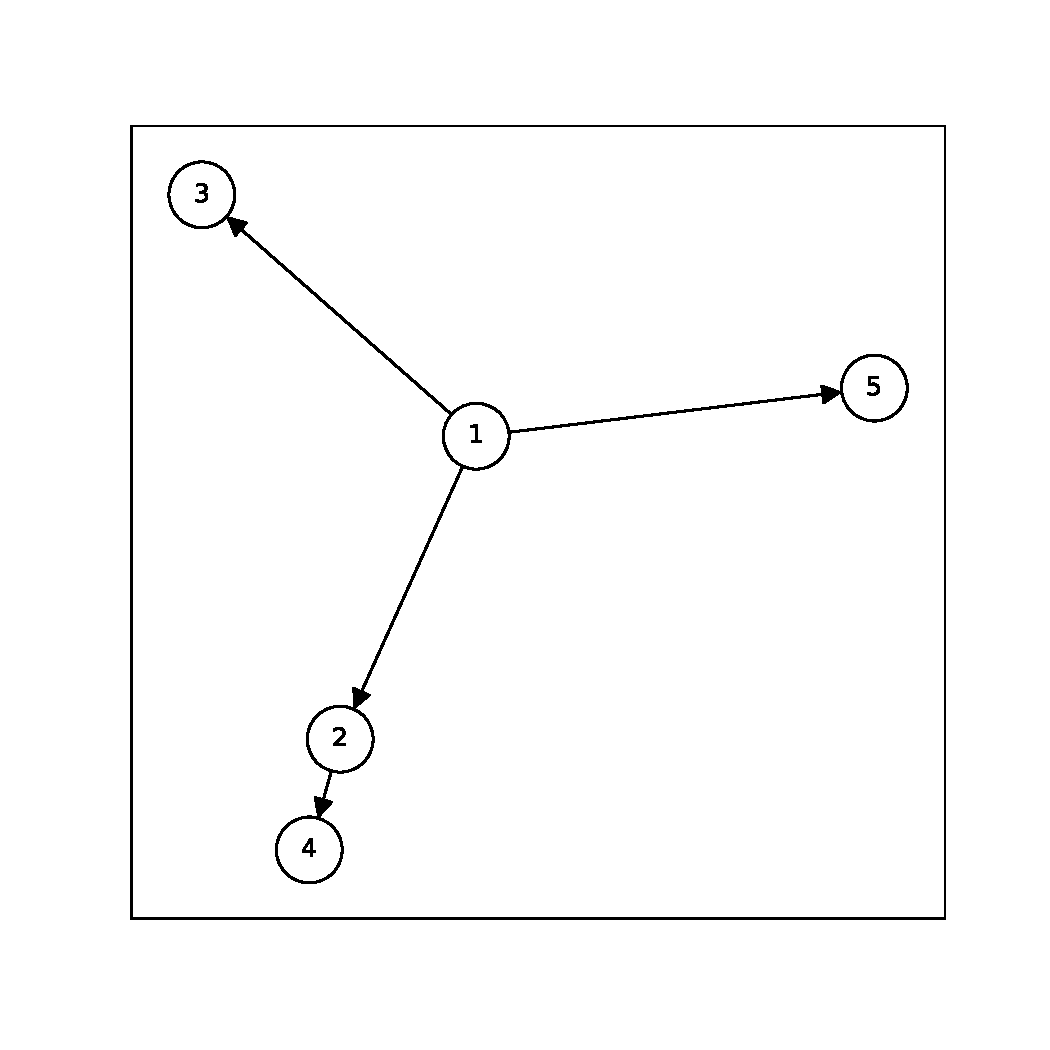
\includegraphics[width=\linewidth]{ ./figures/dageg.pdf}\caption{ Example of a DAG $\mathbb{G}=(\mathbb{V},\mathbb{E})$ with $\mathbb{V} = \{1,2,3,4,5 \}$ and $\mathbb{E} = \{(1,2),(1,3),(1,5),(2,4) \}$} \end{marginfigure} 

 \begin{marginfigure} 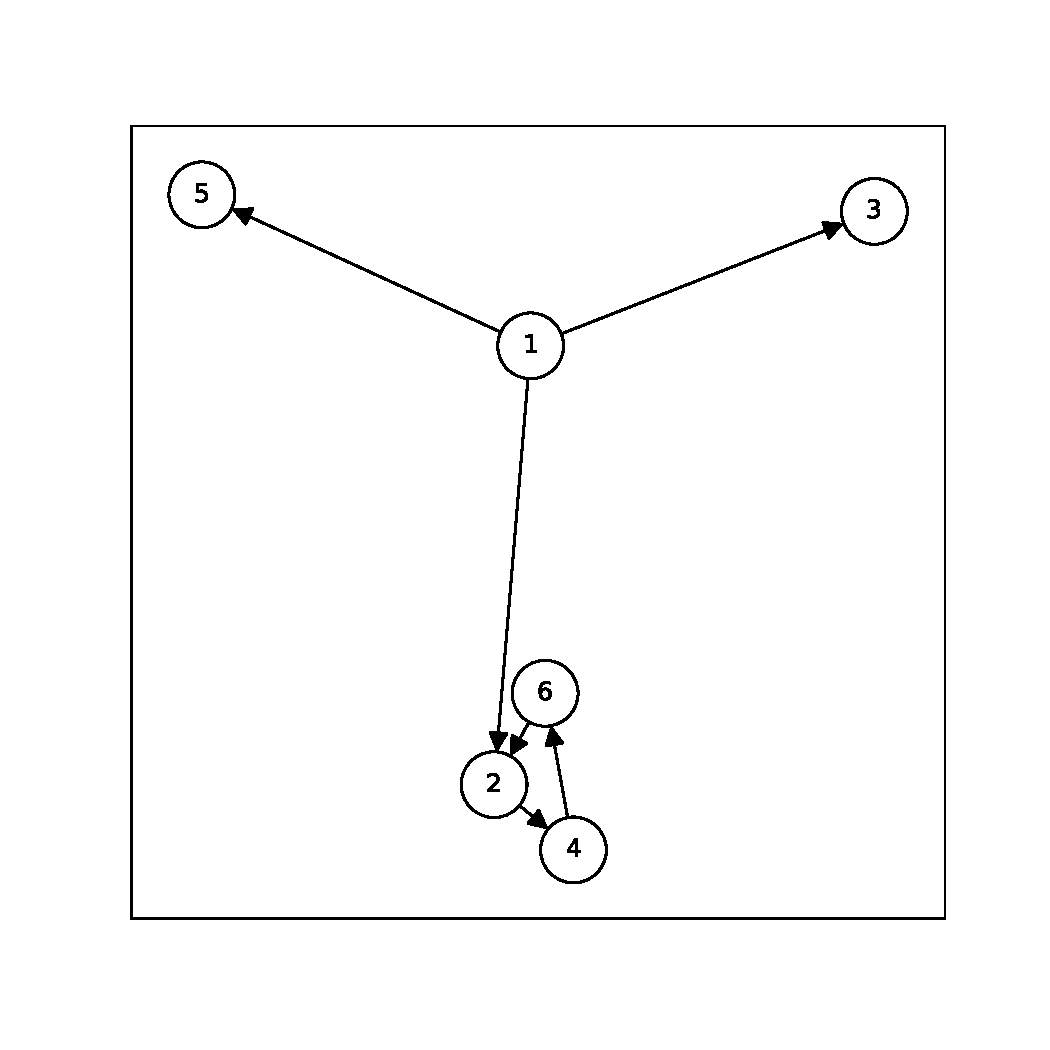
\includegraphics[width=\linewidth]{ ./figures/dagneg.pdf}\caption{ This graph is not a DAG since there is a cycle} \end{marginfigure} 


Since we a working with discrete probability distributions, we introduce the (open) probability simplex as the space of all possible probability distributions over a set of discrete variables \(X_1,...,X_p\) whose outcomes are elements of \(\mathcal{X}=\prod_{i=1}^p \mathcal{X}_i\).

\begin{definition}[Probability simplex]\label{probsimplex}
Given a finite set $\mathcal{X}$, The probability simplex on this set is \\ $\Delta_{|\mathcal{X}|-1} = \{ (f_x \, : x \in \mathcal{X}) \in \mathbb{R}^{|\mathcal{X}|} \, : \, \forall x \in \mathcal{X} \; f_x > 0, \, \sum_{x\in \mathcal{X}}f_x =1\} $
\end{definition}

Each point in the probability simplex corresponds to a joint distribution over \((X_1,...,X_p)\), and our interest mainly lies to the subset of of this space which are connected to structures we can use to model causal relations.


An important concept when relating DAGs to distributions is that of conditional independence, which we define below.
\begin{definition}[Conditional Independence]\label{def:cirel}
Let  $\mathbb{P}$ be a distribution with variables $X_1,...,X_p$. Given non-empty subsets $A,B \subset [p]$ and a (possibly empty) subset $S \subset [p]$ such that $\mathbb{P}(X_B, X_S)>0$ and $A \cap B \cap S = \{\}$, we say the variables $X_A$ and $X_B$ are conditional independent given $S$, (denoted $(X_A\indep_{\mathbb{P}} X_B \,|\, X_S)$) if $\mathbb{P}(X_A, \,|\,X_B, X_S) = \mathbb{P}(X_A \, |\, X_S)$ holds for all possible outcomes of $X_A,X_B,X_S$.
\end{definition}

The conditional independence statement \((X_A \indep_{\mathbb{P}} X_B \,|\,X_S)\) can be viewed as a ternary relation on \(X_A,X_B,X_S\), and is called a Conditional Independence (CI) relation. This relation formalizes the concept of \(X_B\) and \(X_A\) not providing any information when we have obsered \(X_S\), which is to say, if we already know \(X_S\), knowing \(X_B\) does not change the probabilities for \(X_A\), and vice versa.


Using this we can now define the local Markov property which relates d-separations in DAGs to CI relations in distributions.

\begin{theorem}[Local Markov property]\label{thm:localmarkovdag}
Let $\mathcal{G}$ be a DAG with nodes $[p]$. A probability distribution $\mathbb{P}$ satisfies the local Markov property with respect to $\mathbb{G}$ if for each node $i \in [p]$, the variable representing that node, $X_i$ is independent of its non-descendants when conditioned on its parents, formally, $(X_i \indep X_{ND_{\mathbb{G}}(i)}\,|\,X_{PA_{\mathbb{G}}(i)})$
\end{theorem}

This formalizes the fact that in order to computationally generate data from a DAG \(\mathbb{G}\), the value of each variable \(X_i \in \mathcal{X}_i\) depends only on the values of the outcomes of its parents in \(\mathbb{G}\). This means that for a (discrete) distribution \(\mathbb{P}\) with \(p\) variables satisfying the Local Markov property, the distribution can be encoded with \(p\) probability tables which give the probabilities for each \(X_i\) taking a value when conditioned on all possible outcomes of its parents. From a storage perspective, this means we have to store \(\sum_{i=1}^p |\mathcal{X}_i| |\prod_{j \in PA_{\mathbb{G}}(i)}\mathcal{X}_j |\) which is significantly smaller than having to store all possible probability values which would require one table with \(|\prod_{i=1}^p |\mathcal{X}_i|\) values. For binary variables assuming \(d\) parents for each variable, this is the difference between \(p2^{d+1}\) and \(p2^p\).


For the purposes of this thesis, it is worth introducing the Ordered Markov property which uses the concept of a linear ordering.  \footnote{For a DAG \mathbb{G} with $p$ nodes a linear ordering is an ordering of the nodes that respects the directions in $\mathbb{G}$ that is each node $i$ always comes after each $j \in PA_{\mathbb{G}}(i)$. It is a also called a topological ordering} 

\begin{theorem}[Ordered Markov Property]\label{orderedmarkov}
Let $\mathbb{G}$ be a DAG and $\pi = \pi_1 \cdots \pi_p$ a causal ordering of $\mmathbb{G}$. A probability distribution $\mathbb{P}$ satisfies the Ordered Markov property with respect to $\mathbb{G}$ if we have $(X_i \indep X_{\{1,...,i-1 \} \textbackslash PA_{\mathbb{G}}(i)}\,|\, X_{PA_{\mathbb{G}}(i)})$ 
\end{theorem}


An important notion in DAGs is that of d-separation and blocked paths.
  \footnote{\baselineskip \baselineskip A path between 2 nodes is any set of edges connecting them irrespective of the direction.} .


\begin{definition}[Blocked path]\label{bpath}

Given a DAG $\mathbb{G}$, and a path between nodes $i,j \in \mathbb{V}$, we say the \textbf{path is blocked} by a (potentially empty) set of nodes $S$ if either of the following hold:
\begin{itemize}
\item Along the path there is a triple of nodes $(x,s,y)$ such that $x \rightarrow s \rightarrow y$, $x \leftarrow s \leftarrow y$, or $x \leftarrow s \rightarrow y$ with $s \in S$
\item Along the path there is a triple of nodes $(x,s,y)$ such that $x \rightarrow s \leftarrow y$ such that $s \notin S$ and no descendants of $s$ are in $S$.
\end{itemize}

\end{definition}


\begin{definition}[d-separation]\label{def:dsep}

Given a DAG $\mathbb{G}$,  two (non-empty) sets of nodes $X,Y$ are \textbf{d-separated} by a (potentially empty) set of nodes $S$ in $\mathbb{G}$, denoted $(X\indep_{\mathbb{G}}Y\,|\,S)$ if all paths between every node in $X$ and every node in $Y$ are blocked by $S$. 

\end{definition}

 \begin{marginfigure} 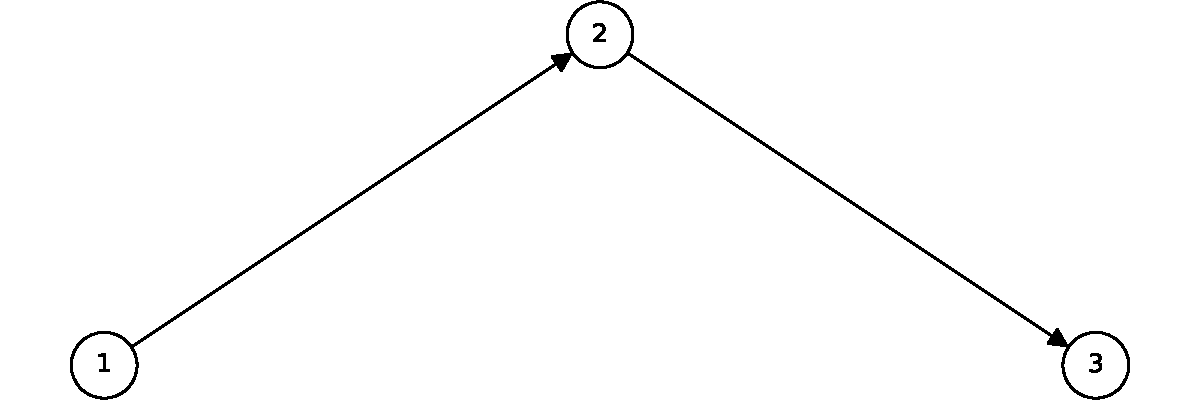
\includegraphics[width=\linewidth]{ ./figures/chainl.pdf}\caption{ Chain} \end{marginfigure} 

 \begin{marginfigure} 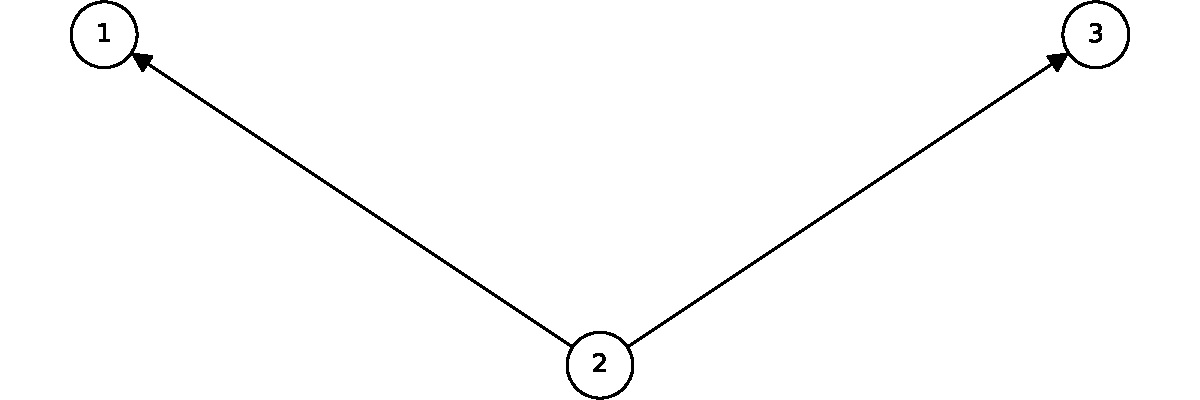
\includegraphics[width=\linewidth]{ ./figures/fork.pdf}\caption{ Fork/Common cause} \end{marginfigure} 
 \begin{marginfigure} 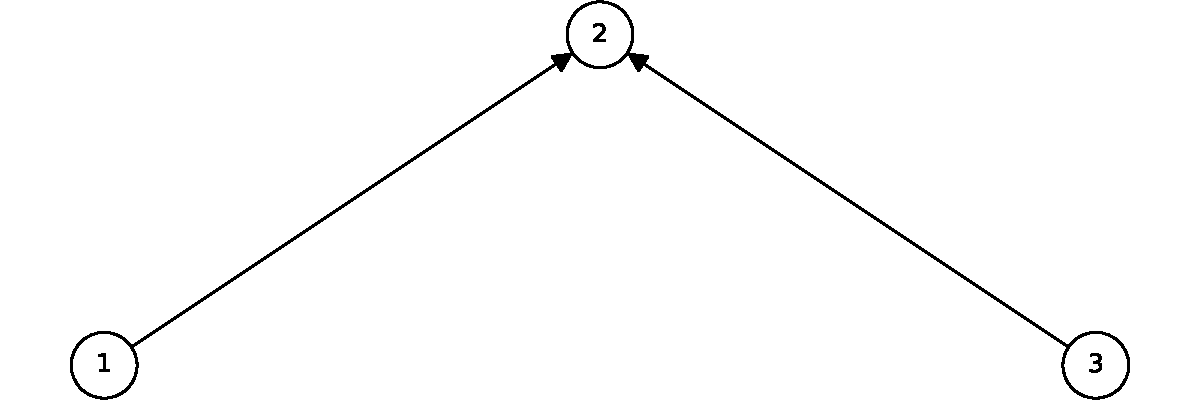
\includegraphics[width=\linewidth]{ ./figures/collider.pdf}\caption{ V-structure/ Collider/Immorality} \end{marginfigure} 


The notion of d-separation relates DAGs to probability distributions from the following theorem.
\begin{theorem}[Global Markov property]\label{thm:dagci}

Given a distribution $\mathbb{P}$ that satisfies the local Markov property with a DAG $\mathbb{G}$, we have that for any (non-empty) sets $A,B$ and (possibly empty) set $S$, $(X_A \indep_{\mathbb{G}} X_B \,|\,X_S) \implies (X_A \indep_{\mathbb{P}} X_B \,|\, X_S)$


\end{theorem}

An important result is the following that the above notions are indeed equivalent \cite{duarte-2020-algeb}.

\begin{theorem}[Markov theorems for DAGs]
Given a distribution $\mathbb{P}$ over $X_1,...,X_p$ and a DAG $\mathbb{G}$ over $p$ nodes, the following are equivalent

\begin{itemize}
\item $\mathbb{P}$ is Markov to $\mathbb{G}$ i.e. $\mathbb{P}(X_1,...,X_p) = \prod_{i=1}^p \mathbb{P}(X_i \, |\, X_{PA_{\mathbb{G}}(i)})$
\item $\mathbb{P}, \mathbb{G}$ satisfy the local Markov property
\item $\mathbb{P}, \mathbb{G}$ satisfy the ordered Markov property
\item $\mathbb{P}, \mathbb{G}$ satisfy the global Markov property
\end{itemize}

\end{theorem}


If \(\mathbb{P}\) satisfies the local Markov property with \(\mathbb{G}\) and has a probability density with respect to a product measure, we say \(\mathbb{P}\) is Markov with respect to \(\mathbb{G}\), or equivalently, \(\mathbb{G}\) is an Independence map (I-MAP) of \(\mathbb{P}\) \cite{lauritzen-1996-graph}. An important result is that 


Thus DAGs can be used to store Conditional Independence (CI) relations. More importantly, d-separation encodes the complete set of CI relations satisfied by all distributions Markov to a DAG, i.e. distributions that are Markov to a DAG \(\mathbb{G}\) \textbf{and} satisfy \textbf{exactly} the CI relations encoded by d-separation exist \cite{meek-2013-stron-compl,geiger1990identifying}.

It is also possible to have 2 DAGs that encode the same CI relations, in which case we say that they are both in the same Markov Equivalence Class (MEC), and we say they are Markov Equivalent. MECs can be characterized by the following theorem \cite{verma-2013-equiv-causal-model}.

\begin{theorem}[Characterization of MECs]\label{thm:vermapearl}
Two DAGs $\mathbb{G}_1$ and $\mathbb{G}_2$ are Markov Equivalent if and only if they have the same skeleton (underlying undirected edges) and v-structures, where a v-structure is a triple of nodes $(i,j,k)$ with edges $i \rightarrow j \leftarrow k$ and $i,k$ do not share an edge.
\end{theorem}

For example, the Chain and Fork graphs from the previous page belong to the same Markov Equivalence class.

\section{Causal Discovery Algorithms for DAGs}
\label{sec:orgec549d5}

Theorem \ref{thm:dagci} suggests that we can make use of CI testing on a distribution \(\mathbb{P}\) to learn a DAG \mathbb{G}. However, the distribution \(\mathbb{P}\) may contain CI relations not encoded in the DAG, thus we make the following assumption.

\begin{definition}[Faithfulness]\label{def:faithfulness}

A probability distribution $\mathbb{P}$ is faithful to a DAG $\mathbb{G}$ if it entails only the CI relations encoded by the d-separations in the DAG.

\end{definition}

Under the faithfulness assumption, Theorem \ref{thm:dagci} holds both ways. It should be noted that faithful distributions exist \cite{meek-2013-stron-compl}, and the set of distributions that are not faithful to a dag \(\mathbb{G}\) have measure 0 \cite{uhler-2013-geomet-faith}, which suggets that in theory this is not a very restrictive assumption.




The PC algorithm \cite{spirtes-2000-causation-prediction-search,kalisch-2007-estim-high} is a constraint based causal discovery algorithm which relies of the characterization of DAGs in Theorem \ref{thm:vermapearl} and the faithfulness assumption to find a DAG in the MEC of the true causal DAG. The algorithm starts from a complete graph and runs conditional independence tests to first find the DAG skeleton and then proceeds to direct the edges whenever possible. The output of the PC algorithm is a Completed Partially Directed Acyclic Graph (CPDAG) \cite{meek-2013-causal-infer}   \footnote{The CPDAG is also sometimes referred to as the Essential Graph or the DAG pattern} , which acts as a representation for the Markov Equivalence class. A Partially Directed Acylic Graph (PDAG) is a graph where some edges are directed and some are undirected and there is no cycle in the direction of the directed edges and any direction of the undirected edges. A PDAG is is Complete PDAG (CPDAG) if every directed edge exists also in every DAG in the Markov Equivalence class of the DAG and for every undirected edge between nodes \(i,j\) there exists a DAG with the edge \(i \rightarrow j\) and a DAG with \(j \rightarrow i\) in the equivalence class.






\section{Limitations of using DAGs}
\label{sec:orga13d919}
DAGs are a simple and informative structure for causal discovery, however their ability to only encode CI relations is a limitation. This is because the CI relation  \((X_A \indep_{\mathbb{P}} X_B \,|\, X_S)\) implies that \(X_A\) and \(X_B\) are independent for all possible outcomes of \(X_S\), which in some cases might be too strong of an assumption. A generalization of such relations is Context Specific Independence (CSI) relations, defined below.
\begin{definition}[Context Specific Independence]\label{def:csirel}
Let  $\mathbb{P}$ be a distribution with variables $X_1,...,X_p$ with a state space $\mathcal{X} = \prod_{i=1}^p \mathcal{X}_i$. Given non-empty subsets $A,B \subset [p]$ and (possibly empty) subsets $S,C \subset [p]$ and $x_C \in \prod_{i \in C}\mathcal{X}_i $ such that $\mathbb{P}(X_B, X_S, X_C = x_C)>0$ and $A \cap B \cap S \cap C = \{\}$, we say the variables $X_A$ and $X_B$ are conditional independent given $S$, in the context $X_C=x_C$ (denoted $(X_A\indep_{\mathbb{P}} X_B \,|\, X_S)$) if $\mathbb{P}(X_A \,|\,X_B, X_S,X_C=x_C) = \mathbb{P}(X_A \, |\, X_S,X_C=x_C)$ holds for all possible outcomes of $X_A,X_B,X_S$.
\end{definition}


In the next chapter we introduce Context Specific Trees (CSTrees) which can encode such relations, and thus provide a structure that can capture the context specific information glossed over in DAGs.


 \newpage 

\chapter{Causal Discovery with Context Specific Trees}
\label{sec:org39ea5e6}
One intuition is that to capture context specific relations one needs to make use of a structure that explicitly represents separate outcomes of a distribution. Typically in high school some might have encountered the use of trees to model small probabilistic systems, and they fully include all possible outcomes involved, and serve as an important tool to compute probabilities for relevant events. As we will see in this chapter, this is a correct way to approach the problem of encoding context information as well.

\section{Context Specific Trees (CSTrees)}
\label{sec:org099f9b1}
Before defining CSTrees we start by defining staged trees, which contain CSTrees as a subset. Both of these are rooted trees.  \footnote{$CH_{\mathbb{G}}$($v$) refers to the set of children of node $v$ in $\mathbb{G}$. A rooted tree $\mathbb{T} = (\mathbb{V},\mathbb{E})$ is a directed graph whose skeleton is a tree and there exists a unique node $r$ such that $PA_{\mathbb{T}}(r) = \{\}$ which is called the root.} 
   \begin{definition}[Staged trees]
   Let $\mathbb{T} = (\mathbb{V},\mathbb{E})$ be a rooted tree, $\mathbb{L}$ a finite set of labels for the edges, and $\theta : \mathbb{E} \rightarrow \mathbb{L}$ a labelling of the edges. Let $E_{\mathbb{T}}(v) = \{v \rightarrow w \in \mathbb{E} \,:\, w \in CH_{\mathbb{T}}(v) \}$,   i.e. the set of edges coming out of $v$ in $\mathbb{T}$. The pair $(\mathbb{T}, \theta)$ is a staged tree if 
\begin{itemize}
\item  $\forall v \in \mathbb{V}$ we have |$\theta(E_{\mathbb{T}}(v))$| = |$E_{\mathbb{T}}(v)$|
\item $\forall v,w \in \mathbb{V}$ we have that both $\theta(E_\mathbb{T}(v))$ and $\theta(E_\mathbb{T}(w))$ are either equal or disjoint
\end{itemize}
\end{definition}

This can be thought of as a probability tree where each edge represents a probability value, and the probabilities coming out of all edges from any given node sum to 1. More formally, first define the space of canonical parameters of the staged tree \((\mathbb{T},\theta)\) as

$\Theta_{\mathbb{T}} = \{  x\in \mathbb{R}^{|\mathbb{L}|} \, : \, \forall e \in \mathbb{E}, x_{\theta(e)}\in (0,1), \forall v \in \mathbb{V} \sum_{e \in E_{\mathbb{T}}(v)} x_{\theta(e)}=1 \}$.

Given the probability simplex \(\Delta_{\mathcal{X}-1}\) and letting \(\mathbf{i}_{\mathbb{T}}\) be the set of all leaves of the staged tree \(\mathbb{T}\)  the staged tree model is defined as below.


\begin{definition}[Staged tree models]\label{def:stagedtreemodel}
The staged tree model $\mathbb{M}_{(\mathbb{T},\theta)}$ is the image of the map $\varphi_\mathbb{T} \, : \, x \rightarrow f_v := (\prod_{e \in E_{\mathbb{T}(\lambda(v))} x_{\theta(e)})_{v \in \mathbf{i}_{\mathbb{T}}}$
\end{definition}

Thus given variables \(X_1,...,X_p\), a causal ordering \(\pi\), the staged tree for this with levels  \footnote{The $k^{th}$ level of a rooted tree, $L_k$, is the set of nodes such that the unique path from each node in $L_k$ to the root consists of $k$ edges.}}} $L_1} 

The important characteristic of staged trees are the stages. 

\begin{definition}[Stages]

Given a staged tree $(\mathbb{T},\theta)$, we say two nodes $v,w$ are in the same stage if and only if  $\theta(E_\mathbb{T}(v)) = \theta(E_\mathbb{T}(w))$

\end{definition}


Stages are represented by colours, and when a stage contains a single node, it is coloured white. Staged tree models generalize DAG models, i.e. distributions represented by DAGs, however they do not take into account the CI relations encoded in them, which arise from the ordered Markov property. Thus we need a structure that generalize DAG models \textbf{and} takes these CI relations into account. A subclass of staged trees, known as CSTrees allow for this, and more importantly, enable us to generalize to the context specific scenario.

\begin{definition}[CSTrees]\label{def:cstree}
Let $\mathcal{X}_i$ denote the state space of some variable $X_i$ with $\mathcal{X} = \Pi_{i=1}^p \mathcal{X}_i$, and $(\mathbb{T},\theta)$ be a staged tree with levels $L_1,...,L_p$ corresponding to variables $X_{\pi_1},...,X_{\pi_p}$ where $\pi = \pi_1...\pi_p$ is the causal ordering of the variables.  
A CSTree is a staged tree $(\mathbb{T}, \theta)$ where each level of the tree corresponds to some variable and  such that 
\begin{itemize}
\item It is compatibly labelled, i.e. $\forall x_{\pi_k} \in \mathcal{X}_i$ we have $\theta(x_{\pi_k}...x_{\pi_{k-1}}\rightarrow x_{\pi_{k-1}}x_{\pi_k}) = \theta(y_{\pi_k}...y_{\pi_{k-1}}\rightarrow y_{\pi_{k-1}}x_{\pi_k})$ whenever $x_{\pi_1}...x_{\pi_{k-1}}$ and $y_{\pi_1}...y_{\pi_{k-1}}$ are in the same stage
\item (\textbf{CSTree property}) Each stage $S_i \subset L_k$ of the tree has a fixed context, i.e. $\exists C_i \subset [k]$ and the fixed outcome context $x_{C_i} \in \mathcal{X}_{C_i}$, where the stages are the union over the variables beside those in $C_i$, i.e. if $Y_i = [k] \textbackslash C_i$ then $S_i = \bigcup_{x_{Y_i} \in \mathcal{X}_{Y_i}} \{x_{C_i}x_{Y_i} \}$  
\end{itemize}
\end{definition}



Given a CSTree \(\mathbb{T}\) and a causal ordering \(\pi\), each node in level \(L_k\) corresponds to an outcome of the sequence of variables \(X_{\pi_1},...,X_{\pi_k}\). Each edge coming into each node in \(L_k\) is of the form \((x_1\cdots x_{k-1},x_1\cdots x_k)\) represents \(P(x_{k}|x_1 \cdots x_{k-1})\). Suppose we fix a node \(n = a_1\cdots a_k \in L_k\). Each edge coming out of \(n\) gives the probabilities for the variable in the next level \(L_{k+1}\), conditioned on the context \((X_{\pi_1}=a_1,...,X_{\pi_k}=a_k)\). Thus, we can view this node \(n\) as containing the distribution \(\mathbb{P}(X_{\pi_{k+1}}\,|\, X_{\pi_1}=a_1,...,X_{\pi_k}=a_k)\) This is an important view which we will make use of when testing for context specific independence in the algorithms throughout this paper. We show an example of a CSTree and a staged tree that is not a CSTree below.

 \newpage 

\begin{figure}[!h]\label{fig:cstreestagedtree}
   \begin{floatrow}
\ffigbox{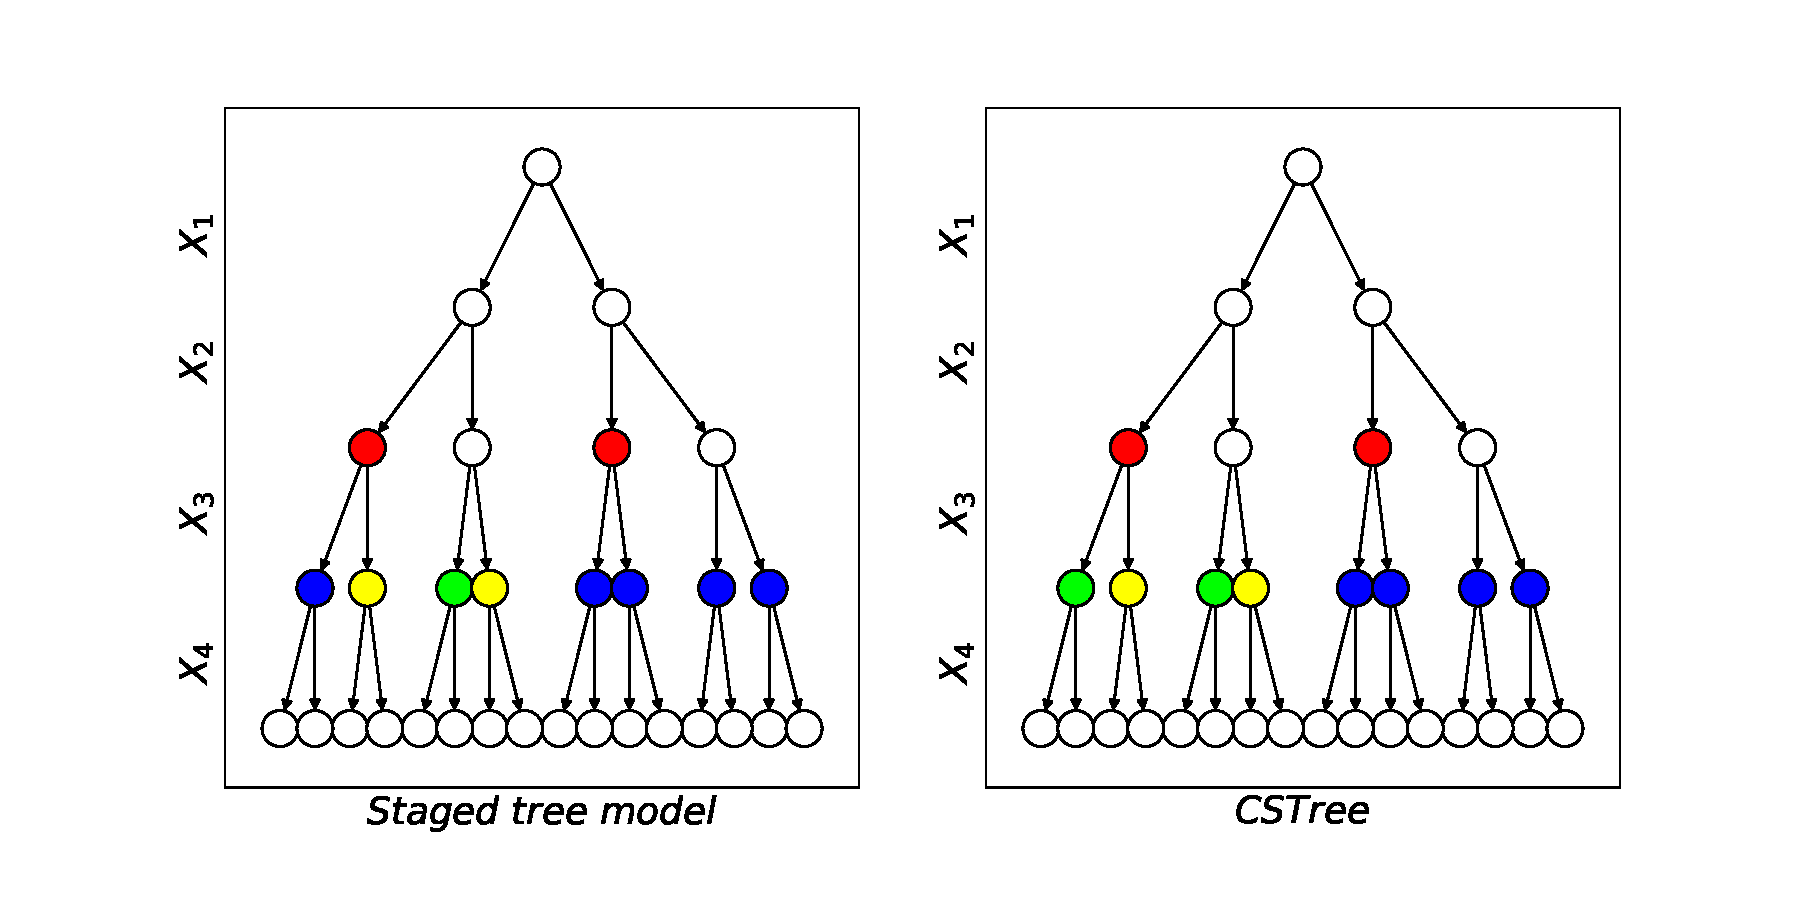
\includegraphics[width=0.95\linewidth]{figures/cstreestagedtree.pdf}}%
\caption{Example of a staged tree model that is not a CSTree (Left) and a CSTree (right) for binary variables $X_1,X_2,X_3,X_4$ in that causal ordering.}
        
   \end{floatrow}
\end{figure}

Both staged trees is Figure \ref{fig:cstreestagedtree} represent 4 binary variables \(X_1,X_2,X_3,X_4\) taking values in \(\{0,1\}\) in that causal order. Suppose each edge to the left corresponds to the outcome 0 and the other corresponds to one. In this case, the left edge coming out of the root represents \(\mathbb{P}(X_1 = 0)\) and the right edge coming out the root represents \(\mathbb{P}(X_1 = 1)\). The nodes represent distributions conditioned on the context unique to them. For example, the left most red node in both trees represent \(\mathbb{P}(X_3 \,|\, X_2=0, X_1=0)\). The tree on the right is a CSTree because each of the nodes in the non-singleton stages, which are represented by a non-white colour, share exactly one fixed context. For example, the stage corresponding to the blue nodes in the tree on the right (the CSTree) corresponds to the contexts \((X_1=1, X_2=0, X_3=0), (X_1=1, X_2=1, X_3=1), (X_1=1, X_2=1, X_3=0), (X_1=1, X_2=1, X_3=1)\). The common context for this stage is  \((X_1=1)\). Meanwhile, for the tree on the left, the stage corresponding to the blue nodes only share the empty context, meaning all nodes in level 3 must correspond to the stage with the empty context for it to be a CSTree.


A CSTree encodes Context Specific Independence (CSI) relations from the following lemma \cite{duarte-2021-repres-learn}


\begin{lemma}[CSTrees and Context Specific Independence relations]\label{lem:cstreecsi}

Let $\mathbb{T} = (\mathbb{V},\mathbb{E})$ be a CSTree with levels $X_1,...,X_p \sim L_1,...,L_p$ and stages $S_1,...,S_m$. Then for any $\mathbb{P} \in \mathbb{M}_{(\mathbb{T},\theta)}$ and $S_i \subset L_{k-1}$, $\mathbb{P}$ entails the CSI relation $(X_k \indep_{\mathbb{P}} X_{[k-1] \textbackslash C_i} \, | \, X_{C_i} = x_{C_i})$ where $X_{C_i}=x_{C_i}$ is the context fixed by the stage $S_i$.

\end{lemma}




\section{Learning CSTrees from observed data}
\label{sec:org2ca5901}
Given a system of variables \(X_1,...,X_p\), we would first need a causal ordering \(\pi_1 \cdots \pi_p\) in order to construct a CSTree for these variables. Since CSTrees encode CSI relations, they can also encode CI relations, which means we can generate a CSTree from a DAG. The following proposition formalizes this notion \cite{duarte-2020-algeb}.

\begin{proposition}[Equivalent DAGs and CSTrees]\label{prop:dagandcstree}
A compatibly labelled staged tree $\mathbb{T}$ with causal ordering $\pi_1 \cdots\pi_p$, levels $L_1,...,L_p$ corresponding to variables $X_{\pi_1},...,X_{\pi_p}$ encodes the same CI relations as some DAG $\mathbb{G}$ if and only if for any topological ordering of $\mathbb{G}$, $\forall k \in [p-1]$, the level $L_k$ has its nodes partitioned into stages where the context for each stage is an element of the Cartesian product of the parents of $X_{\pi_{k+1}}$ in $\mathbb{G}$.
\end{proposition}

We describe the computational procedure to generate a CSTree \(\mathbb{T}\) from a DAG \(\mathbb{G}\) below, assuming that we are given a causal ordering of \(\mathbb{G}\).  \footnote{\textsc{Parents} is a function that takes a graph and a node and returns the parents of that node in the graph; \textsc{CartesianProduct} takes a set of variables and returns the cartesian product of these variables i.e. all possible values they can take} .



\begin{algorithm}[H]
\label{alg:dagtocstree}
      \SetAlgoLined
      \KwIn{A DAG $G$, causal ordering $O$}
      \KwOut{CSTree $T$ with ordering $O$ and stages $S$ defined by $G$}
      $T \leftarrow$ Empty staged tree with ordering $O$\;
      $S \leftarrow$ Empty dictionary\;
       \For{$l$ in $|O|-1$}{
        $v \leftarrow O[l+1]$ \;
	$T.add\_level(v)$\;
	$a \leftarrow \;  \textsc{Parents}(G, v)$\;
	$b \leftarrow$ \textsc{CartesianProduct}($a$)\;
	\tcp{Each element of $b$ is a context which fixes a stage in level $l$}
	\For{$c$ in $b$}{
	$S[c] \leftarrow$ [nodes in level $l$ such that $c$ is a subcontext]\;
	}
       }
       \caption{\textsc{DagToCSTree}\\Constructing a CSTree from a DAG}
       \KwRet{$T, S$}
      \end{algorithm}

Algorithm \ref{alg:dagtocstree} above does not necessarily need a causal ordering since given a DAG we can perform a topological sort on it to get one.

\begin{theorem}\label{thm:dagtocstreecorrectness}
Given variables $X_1,...,X_p$ taking values in $\mathcal{X}=\prod_{i=1}^p \mathcal{X}_i$ , Algorithm \ref{alg:dagtocstree} is correct and runs in $\mathcal{O}(d^{2p})$ time and $\mathcal{O}(d^p)$ space where $d = \max_{i \in [p]} |\mathcal{X}_i|$.
\end{theorem}

\textit{Proof:
	For correctness, at each level $L_k$, the non-singleton stages are created for the contexts fixed by the outcomes of the parents of $X_{\pi_{k+1}}$ thus by Proposition \ref{prop:dagandcstree} the tree is still a CSTree. Since the staging process at each level only creates non-singleton of nodes within that level, and we go over each level except the last level which always contains singleton stages, the stages $S$ lead to $T$ being a CSTree. For time complexity, the worst case scenario is for the fully connected DAG, assuming the ordering $(1,2,...,p)$, node $i$ has $i-1$ parents. This however results in a CSTree with no non-singleton stages. Thus we look at the scenario where node $i$ has $i-2$ parents. At the level for the variable representing node $i$, the variable b in Algorithm \ref{alg:dagtocstree} which is all the elements of the the Cartesian product of values the parents take, has $|\prod_{j=1}^{i-2} \mathcal{X}_j|$ elements. For each element in this Cartesian product which fixes the context for the stage, we have to loop over all nodes in level $i$ and to store the nodes for that stage, and level $i$ has $|\prod_{j=1}^i \mathcal{X}_j|$ nodes. Thus the loop for level $i$ takes $|\prod_{j=3}^{i-2} \mathcal{X}_j ||\prod_{j=1}^i \mathcal{X}_j| $ where the indexing starts at 3 for the first term since the parent sets are non-empty starting from node 3. Since we have $p$ levels, ignoring the first 2 since their variables have no parents, we have $\sum_{i=3}^p |\prod_{j=3}^{i-2} \mathcal{X}_j ||\prod_{k=1}^i \mathcal{X}_k| < \sum_{i=1}^p |\prod_{j=1}^i |\mathcal{X}_j||\prod_{k=1}^i |\mathcal{X}_k|< \sum_{i=1}^p \prod_{j=1}^i d \prod_{k=1}^i d $ where $d = \max_{i \in [p]} |\mathcal{X}_i|$. This sum then becomes $\sum_{i=1}^p d^{2i}  = \frac{d^2 (d^{2p}-1)}{d^2-1} = \mathcal{O}(d^{2p})$. For space complexity, in the worst case DAG mentioned, level $i$ which has $\prod_{j=1}^i |\mathcal{X}_j| < d^i$ nodes and the same amount of edges coming in. For storing the stages, the extra information we need to store is the fixed contexts for each stage, and  there are $\prod_{j=3}^i |\mathcal{X}_j| < d^i$ stages in level $i$, thus the nodes, edges and stages for level $i$ are atmost $3d^i$, summing for each level gives $\sum_{i=1}^p 3d^i= \frac{3d (3d^{p}-1)}{3d-1} = \mathcal{O}(d^{p})$
}

We mention the space complexity here to emphasize that it grows exponentially, which is one limitation of this approach. For \(p\) binary variables this means a CSTree takes \(\mathcal{O}(2^p)\) space. This is in comparison to DAGs which in the worst case assuming full connectivity require \(\mathcal{O}(p^2)\) space, independent of the state space of the variables. 


In order to learn CSI relations, one can now take a CSTree from a DAG and perform statistical CSI testing. Recall that each node in level \(k\) represents a probability density of the variable in level \(k+1\) under the context fixed by that node. Thus for each level, we can compare all possible pairs of nodes by taking the samples fixed by each pair, and testing whether they are from the same distribution. If so, we assign the same colour to both of them. Then by the CSTree property from Definition \ref{def:cstree} we must have that all nodes in level \(k\) which share the same context as that of these 2 nodes must also have the same colour. For example with binary variables we have 2 nodes representing the outcomes \(X_{\{1,2,3,4\}}=0110, X_{\{1,2,3,4\}}=0011\)  \footnote{$X_{\{1,2,3,4\}}=0110$ is shorthand for $(X_1=0, X_2=1, X_3=1,X_4=0)$}   and we know they are in the same stage \(S_i\), then the common context for that stage is \(X_{\{1,4\}}=01\), and by the CSTree property all nodes in that level with this subcontext belong to the same stage. 


 \newpage 
We now describe the algorithm for learning a CSTree.  \footnote{\textsc{Colour} is a function that takes a node and returns the colour of it if it belongs to a non-singleton stage - note here we represent the stage using a colour; \textsc{CommonContext} is a function that takes 2 nodes and returns their common context - if one or both of them already belong to a stage, we take this to be the common context between these contexts; \textsc{Test} is a function that determines whether the distributions corresponding to both of the nodes belong to the same stage or not - this typically involves a statistical test; \textsc{NodesWithContext} takes a set of nodes and a context $c$ and returns the nodes which have the $c$ as a subcontext; \textsc{UpdateStages} is a function that updates the stages of the tree with the new nodes.} 

\begin{algorithm}[H]\label{alg:learncstree}
\SetAlgoLined
\KwIn{CSTree $T$, (possibly empty) stages $S$, causal ordering $O$, Data matrix $D$}
\KwOut{The CSTree $T$ with ordering $O$ and stages $S$}
$l=1$\;
$p=|O|$\;
\While{l < $p$}{
    $ns \gets$ [nodes in level $l$ of $T$]\;
    $ps \gets$ [all pairs of nodes in level $l$]\;
    \For{ $(n_1,n_2)$ in $ps$}{
    \eIf{\textsc{Colour}($n_1$)=\textsc{Colour}($n_2$)}
        {skip}
	{
    $c \gets$ \textsc{CommonContext}($n_1,n_2$)\;
    $same\_distr =$ \textsc{Test}($c, n_1,n_2, \: D, \: O[l+1]$)\;
    \If{same\_distr}
    {
        $new\_nodes \gets$ \textsc{NodesWithContext}($ns,c$)\;
	$S \gets$ \textsc{UpdateStages}($S$, $c$, $new\_nodes$)\;
    }
    }
}
$l=l+1$\;
}
\caption{\textsc{LearnCSTree} \\ Learning a CSTree with knowledge of causal ordering}
\KwRet{$T,S$}
\end{algorithm}

Algorithm \ref{alg:learncstree} can be sped up by already providing a non-empty CSTree containing stages which we may have inferred from a DAG. If one knows the DAG and the true causal ordering of the system they can learn a CSTree by using Algorithm \ref{alg:dagtocstree} followed by Algorithm \ref{alg:learncstree}.


\begin{theorem}\label{thm:learncstreecorrectness}
Given variables $X_1,...,X_p$ taking values in $\mathcal{X}=\prod_{i=1}^p \mathcal{X}_i$ , Algorithm \ref{alg:learncstree} is correct and runs in $\mathcal{O}(d^{2p})$ time assuming constant time for statistical independence testing, where $d=\max_{i \in [p]}\mathcal{X}_i$.

\end{theorem}

\textit{Proof:
For correctness, at level loop iteration we compare all pairs of nodes and only update the stages if they do not belong to the same non-singleton stage. In this case if they do belong to the same stage according to the statistical testing, we add exactly the nodes that belong to the stage according to the CSTree property. Thus the CSTree property is intact throughout the algorithm. For time complexity, using notation from Theorem \ref{thm:dagtocstreecorrectness}, level $i$ has $d^i$ nodes and in the worst case we run statistical testing on all pairs of nodes, of which there are ${d^i \choose 2} = \frac{d^i !}{2! (d^i - 2)!} < \frac{d^{2i}}{2}$, summing for each level gives $\sum_{i=1}^p \frac{d^{2i}}{2}  = \mathcal{O}(d^{2p})$.
}

In the general case it is possible that the true causal ordering is unknown. In fact, we need to consider the set of all causal orderings for each DAG in the MEC of the true DAG. Thus we first learn the CPDAG of the true underlying DAG using the PC algorithm and then apply Algorithms \ref{alg:dagtocstree} and \ref{alg:learncstree}.

\begin{algorithm}\label{alg:cstreepc}
\SetAlgoLined
\KwIn{Data matrix $D$, (optional causal ordering $O$)}
\KwOut{List of CSTrees $T$ with minimum number of stages}
$CPDAG \gets$ \textsc{PcAlgorithm}($D$)\;
\uIf{$O$ given}
{
$G \gets g \in CPDAG$ with ordering $O$\;
$dags \gets$ [$G$]\;
$orderings \gets [O]$\;
}
\uElse{
$dags \gets $ [$g$ in CPDAG]\;
}
$min\_stage\_trees \gets []$\;
$min\_stage \gets \infty$\;
\For{$G$ in $dags$}{


\If{$O$ not given}{
    $orderings \gets$  \textsc{AllTopologicalSort}($G$)\;}

    \For{$O$ in $orderings$}{
    $S,T \gets $ \textsc{DagToCSTree($G$,$O$)}\;
    $S,T \gets $ \textsc{LearnCSTree($T,S,O,D$)}\;
    \If{$|S|$ < $min\_stages$}
    {
    $min\_stages \gets$ |S|\;
    $min\_stage\_trees \gets$ [($T,S$)]\;
    }
    \If {$|S| = min\_stages$}{
    $min\_stage\_trees.append((T,S))$\;}

    

}
}
\KwRet{$min\_stage\_trees$}
\caption{\textsc{CSTreePcAlgorithm} \\ Learning a CSTree from observational data}

\end{algorithm}


We consider all topological orderings of all Markov equiavalent DAGs learnt by the PC algorithm because we might not be able to encode some context specific information otherwise. We show an example of this in the next section after introducing minimal context DAGs.

Algorithm \ref{alg:cstreepc} considers many possible candidate CSTree models, thus we have to pick the best model with respect to some criterion. There are however many instances where we could know the causal ordering apriori \cite{thwaites-2010-causal-analy,silander-2013}, for example a temporal relation between nodes known through physical laws. In this case we can either start statistical testing from an empty tree, or apply the PC algorithm to the data and find a DAG in the Markov Equivalence class with the known ordering and then run the extra testing.



Unlike DAGs, as the number of variables increase it gets progessively harder to visually understand the learnt causal structure by just looking at the learnt CSTree. 

\section{Understanding high-dimensional CSTrees}
\label{sec:org72d6d48}
 From a pragmatic perspective the aim of this section is to introduce the notion of Minimal Context (MC) DAGs which can help visualize CSTrees with more variables and the context specific information they encode. On a theoretical note, this work has led to
the generalization of Theorem \ref{thm:vermapearl} to define a characterization of Markov Equivalence for CSTrees \cite{duarte-2021-repres-learn}. We start by first describing the procedure  \footnote{\textsc{StagesInLevel} takes a set of stages and a level and returns the stages in that level; \textsc{ContextOfStage} takes a stage and returns the common context of that stage; \textsc{VariablesOfContext} takes a context and returns the variables in it}  to generate the CSI relations from a CSTree and its stages, which uses Lemma \ref{lem:cstreecsi}

   \begin{algorithm}\label{alg:gencsirels}
  \SetAlgoLined
  \KwIn{CSTree $T$, its stages $S$ and its causal ordering $O$}
  \KwOut{Set of CSI Relations $J$ encoded in the CSTree}
  $l=1$\;
  $p=|O|$\;
  $J = []$\;
  \While{$l<p$}{
  $S_l \gets $ \textsc{StagesInLevel($S,l$)}\;
  \For{$s$ in $S_l$}{
  $c \gets $ \textsc{ContextOfStage}($S$)\;
  $v_c \gets $ \textsc{VariablesOfContext}($c$)\;
  $v_o \gets O[1:l-1] \textbackslash v_c$\;
  $J.append((X_{O[l+1]} \indep X_{v_o} \, | \, c))$
  % \tcp{Note here $c$ is a variable representing a context}
     }
  }
  
\caption{\textsc{GenerateCsiRelations} \\ Generate the CSI Relations from the CSTree}

   \end{algorithm}


\begin{theorem}\label{thm:gencsirelscorrectness}
Given a CSTree $\mathbb{T}$, Algorithm \ref{alg:gencsirels} is correct and returns the CSI relations encoded in $\mathbb{T}$ in $\mathcal{O}(pd^{2p})$ time.
\end{theorem}
\textit{Correctness follows directly from Lemma \ref{lem:cstreecsi} since at each loop we add exactly the CSI relations mentioned inthe lemma, and we do this for all levels thus include all stages of the CSTree. For time complexity, for each level we first get the stages associated with it, which can be done in constant time if we store this information. We know from the Proof of Theorem \ref{thm:dagtocstreecorrectness} that the number of stages in level $i$ is bounded above by $d^i$, and for each stage in that level we get the context of the stage, which can be done as a constant lookup operation, and we get relevant variables in Lines 8,9 which is bounded above by $2p$. Thus adding this for all the levels give $\sum_{i=1}^p 2pd^i = \mathcal{O}(pd^{2p})$
}


In practice a slightly modified version of Algorithm \ref{alg:gencsirels} can be placed a subroutine in the previous algorithms right before moving onto the next level.


From Lemma \ref{lem:cstreecsi} we know any distribution in the CSTree model \(\mathbb{M}_{(\mathbb{T},\theta)}\) encodes the CSI relations of the given form, there could be more CSI relations satisfied by every distribution in \(\mathbb{M}_{(\mathbb{T},\theta)}\), which is similar to how a DAG model encodes the CI relations \(\mathbb{J}_1\) implied by the local Markov property, on top of the CI relations \(\mathbb{J}_2\) from the global Markov property (i.e. rom the d-separations), and \(\mathbb{J}_1 \subset \mathbb{J}_2\).


We call a collection of CSI relations a Context Specific Conditional Independence model \(\mathbb{J}\). The complete of set of all CSI relations satisfied by each distribution \(\mathbb{P} \in \mathbb{M}_{(\mathbb{T},\theta)}\) includes the CSI relations recovered from Algorithm \ref{alg:gencsirels}, and also include those implied by the succesive application of the Context Specific Conditional Independence axioms to generate further CSI relations. The axioms are as follows


\begin{enumerate}
\item Symmetry, If \((X_A \indep X_B \,|\, X_C=x_c) \in \mathbb{J}\) then \((X_B \indep X_A \,|\, X_c=x_c) \in \mathbb{J}\)
\item Decomposition, If \((X_A \indep X_{B \cup D} \,|\, X_S, X_C=x_c) \in \mathbb{J}\) then \((X_A \indep X_B \,|\, X_S, X_C=x_c) \in \mathbb{J}\)
\item Weak union, If \((X_A \indep X_{B \cup D} \,|\, X_S, X_C=x_c) \in \mathbb{J}\) then \((X_A \indep X_{B} \,|\, X_{S \cup D}, X_C=x_c) \in \mathbb{J}\)
\item Contraction, If \((X_A \indep X_B \,|\, X_{S \cup D}, X_C=x_c) \in \mathbb{J}\) and \((X_A \indep X_D \,|\,X_S, X_C=x_c) \in \mathbb{J}\) then \((X_A \indep X_{B \cup D} \,|\, X_S, X_C=x_c) \in \mathbb{J}\)
\item Intersection,  If \((X_A \indep X_B \,|\, X_{S \cup D}, X_C=x_c) \in \mathbb{J}\) and  \((X_A \indep X_B \,|\, X_{B \cup D}, X_C=x_c) \in \mathbb{J}\) then  \((X_A \indep X_{B \cup S} \,|\, X_D, X_C=x_c) \in \mathbb{J}\)
\item Specialization, If \((X_A \indep X_B \,|\, X_S, X_C=x_c) \in \mathbb{J}\) and \(T \subset S, x_T \in \mathcal{X}_T\) then \((X_A \indep X_B \,|\, X_{S \textbackslash T}, X_{T \cup C} = x_{T \cup C}) \in \mathbb{J}\)
\item Absorption, If \((X_A \indep X_B \,|\, X_S, X_C=x_c) \in \mathbb{J}\) and \(\exists T \subset C\) such that \(\forall x_T \in \mathcal{X}_T\) we have \((X_A \indep X_B \,|\, X_S, X_{C\textbackslash T}=x_{C \textbackslash T}, X_T=x_T) \in \mathbb{J}\) then \((X_A \indep X_B \,|\, X_{S \cup T}, X_{C \textbackslash T}=x_{C \textbackslash T}) \in \mathbb{J}\)
\end{enumerate}


Given a Context Specific Conditional Independence model \(\mathbb{J}\), the successive application of the axioms above results in the Context Specific closure  of the model, denoted \(\mathbb{\overline{J}}\)


The Absorption axiom helps us to get a representation of the CSTree as a sequence of DAGs. For this we need the definition of minimal contexts \cite{duarte-2021-repres-learn}.
\begin{definition}[Minimal contexts]\label{def:mcs}
Given a set Context Specific Independence model $\mathbb{J}$, we say that ${X_C=x_C}$ is a minimal context if we have $(X_A  \indep X_B \,|\, X_S, X_C=x_C) \in \mathbb{J}$ and there is no non-empty subset $T \subset C$ such that $(X_A \indep X_B \,|\, X_{S \cup T}, X_{C \textbackslash T}=x_{C\textbackslash T}) \in \mathbb{J}$.
\end{definition}

Intuitively, the minimal contexts are the smallest contexts that get left behind after repeated application of the Absorption axiom. By the Specialization axiom, given a minimal context \((X_C=x_C)\) we can recover all the CI relations implied by the CSTree. We give some examples of minimal contexts below.

\begin{example}\label{eg:mc1}
Let $X_1,X_2,X_3,X_4,X_5$ be binary variables taking values in $\{0,1\}$. If we have just the CSI relations $(X_5 \indep X_4 \,|\, X_{\{1,2,3\}}=000)$ and $(X_5 \indep X_4 \,|\, X_{\{1,2,3\}}=100)$ they get absorbed into $(X_5 \indep X_4 | X_{\{1\}}, X_{\{2,3\}}=00)$ leaving the minimal context $X_{\{2,3\}}=00$, or simply $(X_2 = 0, X_3=0)$  
\end{example}

\begin{example}\label{eg:mc2}
Let $X_1,X_2,X_3,X_4$ be binary variables taking values in $\{0,1\}$. If we have the  CSI relations $(X_4 \indep X_2 \,|\, X_{\{1,3\}}=00), $\\$ (X_4 \indep X_2 \,|\, X_{\{1,3\}}=01), (X_4 \indep X_2 \,|\, X_{\{1,3\}}=10), (X_3 \indep X_1 \,|\, X_2=1)$ then they absorb to give the equivalent CSI relations $(X_4 \indep X_2 \, |\,X_1, X_3=0), (X_4 \indep X_2 \,|\, X_3, X_1=0), (X_3 \indep X_1 \,|\,X_2=0)$ thus the minimal contexts are $(X_1=0),(X_2=0),(X_3=0)$
\end{example}

Example \ref{eg:mc1} shows that we can get absorption from CSI relations we get from different levels, while \ref{eg:mc2} shows that we have to check at least all possible pairs of CSI relations to get the minimal contexts. It is also possible to get the empty context as the minimal context, which happens when the all CSI relations \((X_A \indep X_B \,|\, X_S, X_C=x_C)\) hold for all outcomes \(x_C \in \mathcal{X}_C\) in which case the absorption axiom gives the CI relation \((X_A \indep X_A\,|\,X_S,X_C)\).


From a computational perspective, given all CSI relations involving sets of variables \(X_A,X_B\) i.e. those of the form \((X_A \indep X_B \,|\, X_S, X_C=x_C)\), we want to find the largest set \(T \subset C\) such \((X_A \indep X_B \,|\, X_S, X_T=x_T, x_{C \textbackslash T} = x_{C \textbackslash T})\) is also in the CSI relations.  \footnote{If we are to use the CSI relations extracted from Algorithm \ref{alg:gencsirels} before getting their Context Specific closure they would be of the form $(X_i \indep X_B | X_C=x_C)$ where $i \in [p]$ and $B ,C \subset [p-1]$}  This can be thought of as decomposing \(C\) into sets \(C \textbackslash T\) and \(T\) such that Definition \ref{def:mcs} holds. To find the largest such \(T\), we can perform a binary search on the size of \(T\), which can range from 0 to \(|C|\).
We describe this method below.  \footnote{Each break statement leaves the first loop it meets.} 
\begin{algorithm}\label{alg:genmcs}
  \SetKw{Break}{break}
  \SetAlgoLined
  \SetKwBlock{Begin}{Begin}{}
  \KwIn{Set of CSI Relations $J$}
  \KwOut{Set of minimal contexts $MCs$ from $J$}
  $set\_pairs \gets$ \textsc{PairsOfSets}($J$),$MCs \gets$ \textsc{EmptyDictionary}\;
  \For{$A,B$ in $set\_pairs$}{
    $rels \gets$ \textsc{RelsOfPair}($A,B$),$cs \gets$ \textsc{ContextsOfRels}($rels$)\;
    \For{$rel$ in $rels$}{
        $C \gets$ \textsc{VariablesOfContext}(\textsc{ContextOfRels}($rel$))\;
        $T\_sizes \gets$ [0,...,|C|],$T\_found=False$\;
        \While{not $T\_found$}{
            $mid \gets |T\_sizes|$/2 , $T\_size \gets T\_sizes[mid]$\;
            $T\_candidates \gets$ [subsets of $C$ of size $T\_size$] \;
            \For {$T$ in $T\_candidates$}{
                $T\_contained \gets False$\;
                $x_{Ts} \gets$ \textsc{CartesianProduct}($T$),
                $x_{Ts}\_count = 0$\;
                \For {$x_T$ in $x_{Ts}$} {
                    $x_{T}\_contained \gets$ True if $x_T$ in $cs$ else False\;
                    \If{$x_{T}\_contained$ is True}{
                        $x_{Ts}\_counts +=1$\;
                        \If{$x_{Ts}\_counts = |x_{Ts}|$}{
                             $T\_contained \gets$ True\;
                         $search\_upperhalf \gets$ True\;
                             }
                       }
                    \If{$x_T\_contained$ is False}{
                    $search\_lowerhalf \gets$ True
                    \Break}

                }
                \If{(T\_contained and |T\_candidates|=1) or T\_sizes=[0] or T\_sizes=[|C|]}{
                    $T\_found \gets True$\;
		$MCs \gets$ \textsc{UpdateMinContexts}($MCs,rels$)\;
                }


                \uIf{search\_upperhalf}
                {T\_sizes = T\_sizes[mid:end]
                \Break}
                \If{search\_lowerhalf}
                {T\_sizes = T\sizes[start:mid]
                \Break}

            }


            \If{T\_found}
            {\Break}
        }
        \If{T\_found}
        {\Break}
    }}
  }\caption{\textsc{GenerateMinimalContexts} \\ Generate the Minimal Contexts from a set of CSI relations}

\end{algorithm}

\begin{theorem}\label{alg:genmcscorrectness}
Given a set of Context Specific Independence relations $\mathbb{J}$, Algorithm \ref{alg:genmcs} returns the set of minimal contexts in [!!! a long time theoretically]
\end{theorem}

[!!! Describe subprocedures in minimal context generator algorithm]

In theory, the number of possible pairs of sets \(A,B\) is \({2^p}\choose{2}\), though in practice it can be reduced, for example by the Symmetry axiom allows us to half the number of pairs we need to check. This motivates us to the pairwise case, where we focus on Context Specific Independence relations of the form between 2 variables \(X_i,X_j\) rather than two sets of variables \(X_A,X_B\). This drops the number of possible pairs to \(p \choose 2\). This leads us to the definition of pairwise minimal contexts.

 \newpage 
\begin{definition}[Pairwise minimal contexts]\label{def:pairmcs}
Given a set Context Specific Independence model $\mathbb{J}$, we say that ${X_C=x_C}$ is a pairwise minimal context if we have $(X_i  \indep X_j \,|\, X_S, X_C=x_C) \in \mathbb{J}$ and there is no non-empty subset $T \subset C$ such that $(X_i \indep X_j \,|\, X_{S \cup T}, X_C=x_C) \in \mathbb{J}$.
\end{definition}

We can make use of the Context Specific Conditional independence axioms to generate pairwise CSI relations to get the pairwise minimal contexts.


The introduction of pairwise relations motivates the inclusion of the following axiom.
\begin{enumerate}
\setcounter{enumi}{7}
\item Composition, If \((X_A \indep X_B \,|\, X_S, X_C=x_C)\) and \((X_A \indep X_D \,|\,X_S,X_C=x_C)\) then \((X_A \indep X_{B\cup D} \,|\,X_S,X_C=x_C)\)
\end{enumerate}


The composition axiom allows us to go from pairwise relations between variables to the more general pairwise relations between sets of variables. We call a Context Specific Conditional Independence model satisfying the additional composition axiom a Context Specific compostional graphoid, which generalizes the notion of compositional graphoids \cite{sadeghi-2014-markov-proper}. An important question is whether the Context Specific closure of CSI relations from a CSTree form a compositional context specific graphoid.


Pairwise minimal contexts are always minimal contexts however but we could have minimal contexts that are not pairwise minimal contexts. If all CSTrees have an associated compositional context specific independence model, the pairwise relations may indeed be all that we need to get the set of complete set of minimal contexts. We leave this as an open question and use pairwise minimal contexts to offer a visualization of CSI relations in the CSTree which may potentially be incomplete.


Denote \(\mathbb{C}(\mathbb{T})\) as the set of all minimal contexts of a CSTree \(\mathbb{T}\), and denote \(\mathbb{G}(\mathbb{T}) := \{ \mathbb{G}_{X_C=x_C} \}_{X_C=x_C \in \mathbb{C}(\mathbb{T})}\) as the set of all minimal context DAGs of \(\mathbb{T}\).

We now have the machinery to visualize higher dimensional CSTrees.We start by generating the CSI relations from the trees. Then get the Context Specific closure, and then get the minimal contexts. Once we have the minimal contexts, the CI relations for each minimal context define a graphoid. This is called a Minimal Context DAG. Thus, the CSTree can be represented as a sequence of DAGs for each minimal context. This representation is a consequence of the following theorem \cite{duarte-2021-repres-learn}.

 \newpage 

\begin{theorem}[Markov theorem for CSTrees]\label{thm:markovtheoremcstrees}
Given a CSTree $\mathbb{T}$, with levels $L_1,...,L_p \sim X_1,...,X_p$, minimal contexts $\mathbb{C}(\mathbb{T})$ and $\mathbb{P} \in \Delta_{\mathcal{X}-1}$. The following are equivalent.
\begin{itemize}
\item $\mathbb{P}$ factorizes according to $\mathbb{T}$.
\item $\mathbb{P}$ is Markov to $\mathbb{G}(\mathbb{T})$.
\item $\forall \, X_C = x_C \in \mathbb{C}(\mathbb{T})$ we have\\ $\mathbb{P}(X_{[p]\textbackslash C}\,|\,X_C=x_C) = \prod_{k \in [p]\textbackslash C} \mathbb{P}(X_k \, |\, X_{PA_{\mathbb{G}_{X_C=x_C}}(k)}, X_C=x_C)$.
\end{itemize}
\end{theorem}


This DAG is also called the minimal I-MAP \cite{verma-1990-causal-networ}, which we can recover with the following procedure \cite{solus-2021-consis-guaran}.


\begin{algorithm}\label{alg:mcdags}
\SetAlgoLined
\KwIn{Causal ordering $O$, Minimal Contexts $MCs$ as a dictionary with minimal contexts as keys and the CI relations under the minimal context as values}
\KwOut{List of minimal contexts with their minimal context DAGs $MCDAGS$}
$MCDAGS \gets []$\;
\For{$MC$, $Ci\_Rels$ in $MCs$}{
$G \gets$ Empty Graph\;
    $nodes \gets O \textbackslash$ \textsc{VariablesOfContext}($MC$)\;
    \For{$i$ in [1,...,|$nodes$|]}{
        \For{$j$ in [$i+1$,...,|$nodes$|]}{
	    $\pi_i \gets nodes[i]$\;
	    $\pi_j \gets nodes[j]$\;
	    $G.add\_edge(\pi_i, \pi_j)$\;
	    $S = O[1:j-1] \textbackslash $\textsc{VariablesOfContext}($MC$) \textbackslash $\{\pi_i\}$ \;

	    \If{$(X_{\pi_i} \indep X_{\pi_j} \,|\, X_S) \in Ci\_Rels$}{
	        $G.remove\_edge(\pi_i,\pi_j)$
	    }
	}
    }


$MCDAGS.add((MC,G))$\;
}

\caption{\textsc{GenerateMinContextDags} \\ Generating minimal context DAGs}
\KwRet{$MCDAGS$}
\end{algorithm}


\begin{theorem}\label{thm:mcdagscorrectness}
Given variables $X_1,...,X_p$, a set of minimal contexts $C$ and for each minimal context $C$ the conditional independence relations $\mathbb{J}_C$ that hold under this minimal context, Algorithm \ref{alg:mcdags} is correct and runs in $\mathcal{O}(p^2 |C||\mathbb{J}|)$ time.
\end{theorem}


%\textit{Proof:
%}



We end this section by stating the definition of faithfulness for CSTrees which allows us to explain why we consider all Markov equivalent DAGs when learning a CSTree, followed by the main theorem for Algorithm \ref{alg:cstreepc}

\begin{definition}[Faithfulness for CSTrees]\label{def:faithfulnesscstrees}
A distribution $\mathbb{P}$ is faithful to a CSTree $\mathbb{T}$ if it entails exactly the CSI relations encoded by the set of minimal context DAGs $\mathbb{G}(\mathbb{T})$.
\end{definition}

To see why we need to consider all Markov equivalent DAGs in Algorithm \ref{alg:cstreepc}, suppose we have the following case with 4 binary variables.


\begin{figure}[!h]\label{fig:dagtocstree_cstree}
   \begin{floatrow}
\ffigbox{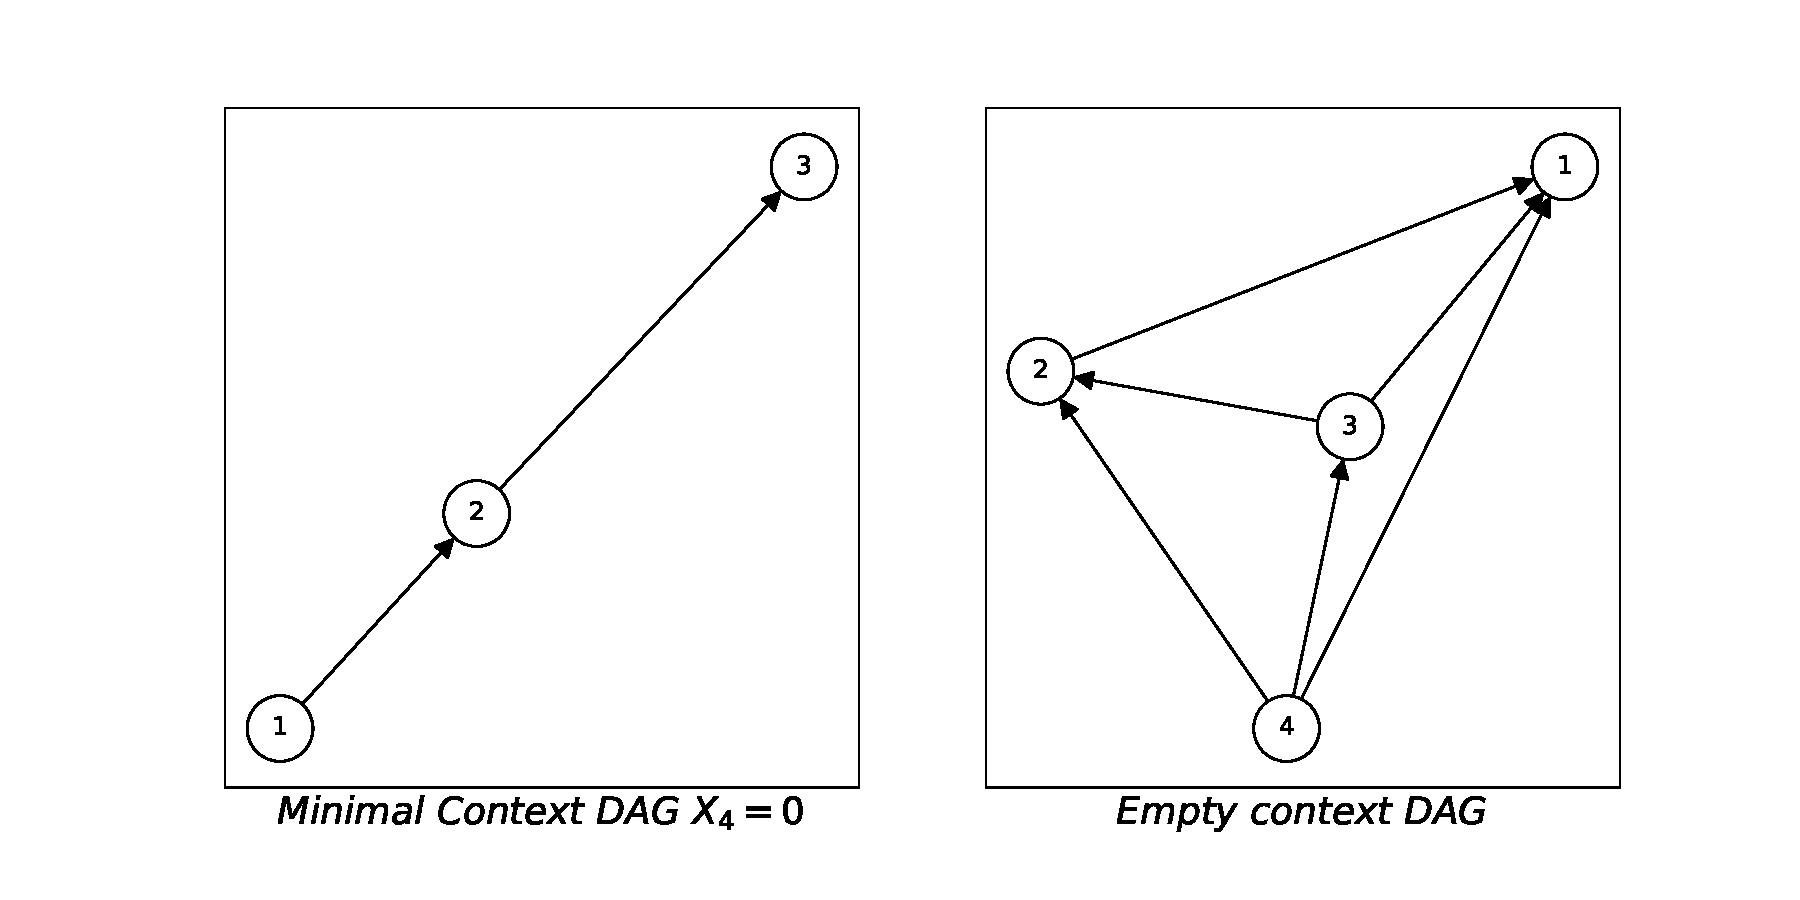
\includegraphics[width=1\linewidth]{figures/exampleonallmec.pdf}}%
\caption{Example on why to consider all topological ordering of all Markov equivalent DAGs when learning a CSTree}
        
   \end{floatrow}
\end{figure}


Let \(\mathbb{P}\) be the data generating distribution and suppose it is faithful to the CSTree with the context graph shown above for the context \(X_4=0\). The empty context DAG could possibly be the fully connected shown above. If we do happen to learn this DAG from the PC algorithm step, it only has one topological ordering which is 4321, and there is no way to join the stages for the empty context graph which this order to encode \((X_1 \indep X_3 \,|\,X_4=0)\), in which case we do not learn the true model.


\begin{theorem}\label{thm:cstreepccorrectness}
Given variables $X_1,...,X_p$, assuming that the data generating distribution is faithful to some unknown CSTree $\mathbb{T}$ with a known causal ordering $\pi = \pi_1 \cdots \pi_p$, Algorithm \ref{alg:cstreepc} is consistent, i.e. it recovers $\mathbb{T}$ as the number of samples $n \rightarrow \infty$.
\end{theorem}


\section{Model selection for CSTrees}
\label{sec:org8f6f51a}
In Algorithm \ref{alg:cstreepc} we select the CSTree (or CSTrees if there is more than one) with the causal ordering corresponding to the fewest stages, which is motivated by the principle of Occams razor since few stages imply lower model complexity and all else being, the simplest model is the best model. The original authors also present the \textbf{Bayesian Information Criterion (BIC)} for CSTrees alongside a proof that it is locally consistent for CSTrees, meaning it can be applicable to greedy search methods for CSTrees. The BIC depends on two terms, the likelihood of the data, which assesses the quality of the model to explain the observed data, and a complexity term that depends on the amount of observed data and the free parameters of the model, with the idea being that models with more parameters should be penalized. Importantly, this helps against overfitting since one can simply add more parameters to the model to maximize the likelihood.


For a general model with random variables \(X_1,...,X_p\) the likelihood of observing a sample \((x_1,...,x_p)\) can be described as below  \footnote{Here we compactify the notation further - $X_{\{1,...,p\}}=x_{\{1,...,p\}}$ is the same as $X_{\{1,...,p\}}=x_1\cdots x_p$ which is $X_1=x_1,...,X_p=x_p$} 
.


\begin{align*}
\mathbb{P}(X_{\{1,...,p\}}=x_{\{1\cdots x_p\}}) =\mathbb{P}(X_i=x_i|X_{\{i-1,...,1\}}=x_{\{i-1,...,1 \}})\\\cdots\mathbb{P}(X_2=x_2|X_1=x_1)\mathbb{P}(X_1=x_1)
\end{align*}

In the CSTree model, independence is implied from the staging of the tree, and each distribution in the product above depends on the fixed context of the node in the CSTree representing that distribution. Denoting \(C_i\) to be the context variables of the context of the node \(x_1\cdotsx_i\), this gives the following.

\begin{align*}
\mathbb{P}(X_{\{1,...,p\}}=x_{\{1,..., p\}}) =\prod_{i=1}^p \mathbb{P}(X_i=x_i|X_{C_i}=x_{C_i})
\end{align*}


In order to get these values from the data, we denote \(\mathbb{U}\) to be \textbf{contingency table} of the data, which a multi-dimensional array  \footnote{This is the same as tensors in the context of computer science}   with dimensions \(d_1 \times \cdots \times d_p\), where \(d_i\) is the number of possible outcomes for variable \(X_i\), and given a sample \((x_1,...,x_p)\), the value in \(\mathbb{U}[(x_1,...,x_p)]\) is the number of times we have this sample in the dataset. The marginalized contingency table \(\mathbb{U}_C\) represents the table after summing over the axes which are not in \(C\). An important case is when \(C\) is the empty set, which results in the marginal table to be 1 dimensional scalar and is the total number of samples in the dataset - when having a stage with an empty context this reflects the conditional distribution for the corresponding variable to simply be the ratio of its outcomes in the dataset. This allows the following compact representation for the likelihood \cite{duarte-2021-repres-learn} for a tree with levels \((L_1,...,L_p) \sim (X_1,...,X_p)\).

\begin{align*}
\mathbb{P}(X_{\{1,...,p\}}=x_{\{1,..., p\}}) = \prod_{k=1}^p \frac{\mathbb{U}_{C \cup k}[x_{C \cup k}]}{\mathbb{U}_{C}[x_{C}]}
\end{align*}

Given \(n\) samples arranged into a \(n \times p\) array \(\mathbb{D}\), and under the assumption that they are independent, the total likelihood is simply the product over all samples in \(\mathbb{D}\).


The free parameters is \(d=\sum_{k=1}^{p-1} (|\mathcal{X}_k| - 1)S_k\) where \(S_k\) is the number of distinct stages in level \(k\) \cite{duarte-2021-repres-learn}. The  BIC score for a CSTree \(\mathbb{T}\) with observed data \(\mathbb{D}\) is then

\begin{align*}
\textbf{BIC}(\mathbb{T},\mathbb{D}) = \log\mathbb{P}(\mathbb{D}\,|\,\mathbb{T}) - \frac{d}{2}\log(n)
\end{align*}



\chapter{Experiments}
\label{sec:org5f6af5a}
The aim of this section is to run test the theory presented so far in both synthetic and real world data. Namely, for all the datasets we use, we ask ourselves the following.
\begin{enumerate}
\item Given a DAG and a causal ordering, is there a difference between learning the context specific independence relations after encoding the CI relations from the DAG into CSTree, or without encoding any of these CI relations?
\item Is the CSTree property assumption reasonable in practice?
\item How sensitive are the results on the method used to determine whether nodes belong to the same stage?
\item How are the results in comparison to CSTrees generated from DAGs learnt using other causal discovery algorithms?
\end{enumerate}


Throughout this section we omit the final layer of nodes for all the CSTrees since they always belong to the singleton stage.


\section{Encoding DAGs as CSTrees}
\label{sec:orgcc85d7e}
We first run a sanity check on generating the CSTrees from DAGs in the 2 extreme cases, when we have no connectivity and full connectivity.

\begin{figure}[!h]\label{fig:dagtocstree_cstree}
   \begin{floatrow}
\ffigbox{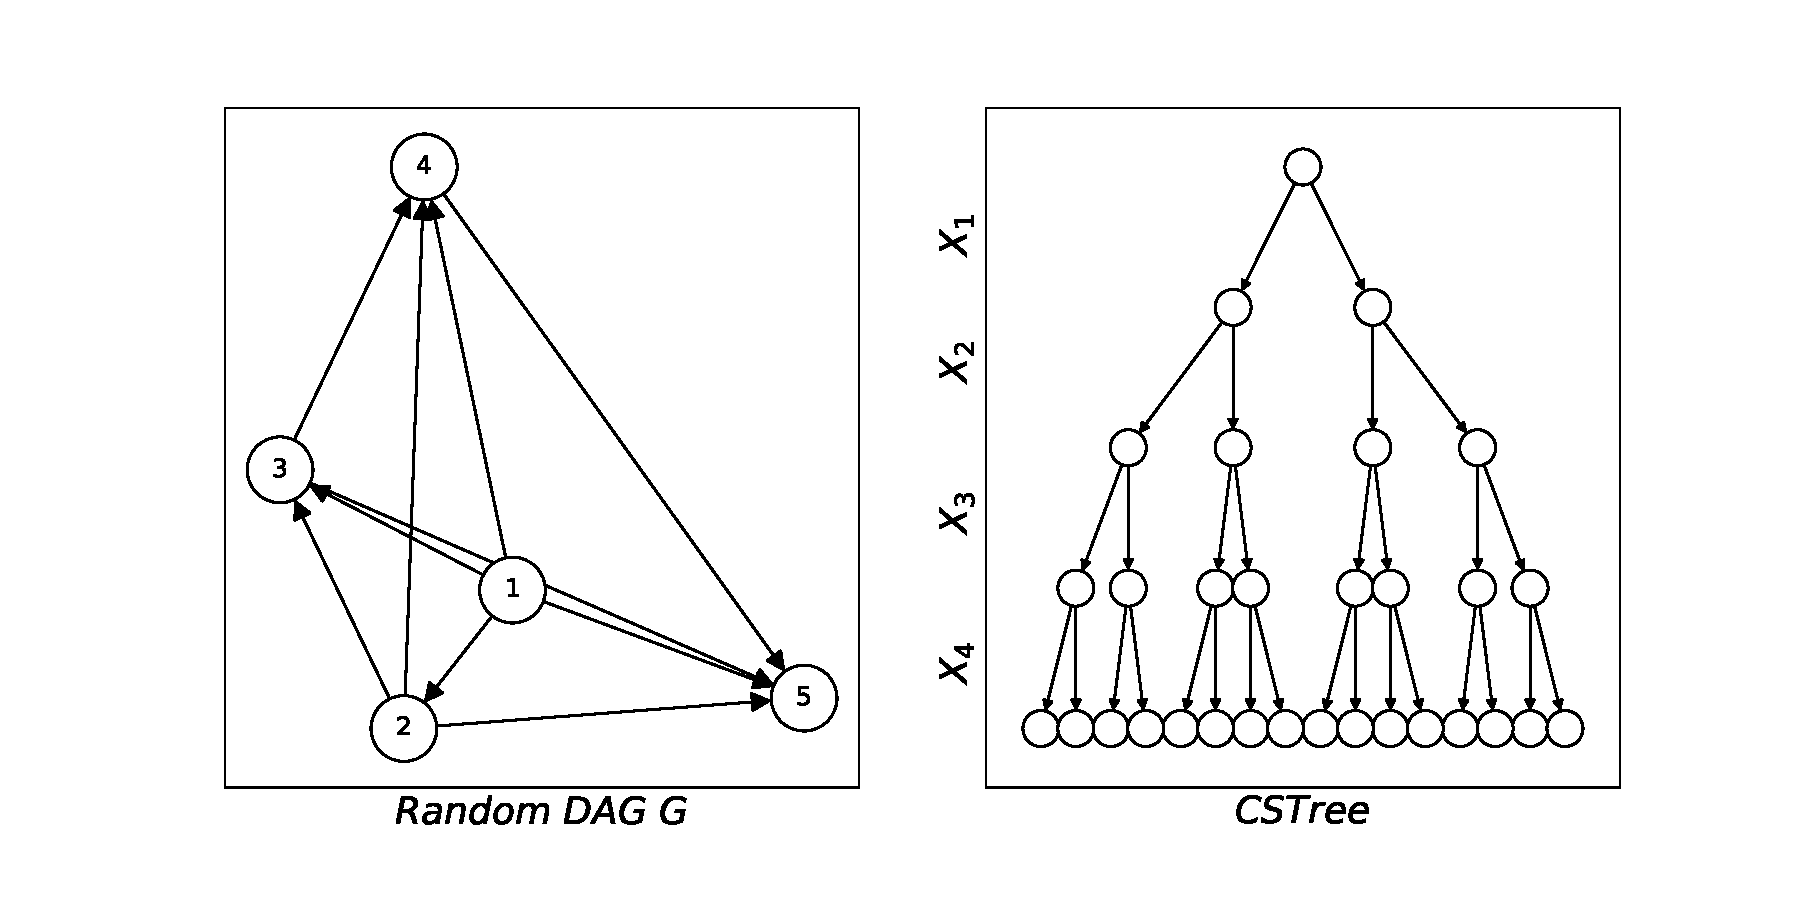
\includegraphics[width=1\linewidth]{figures/fulldagtocstree.pdf}}%
\caption{Generating the CSTrees for a fully connected DAG using the ordering 1234 with Algorithm \ref{alg:dagtocstree}}
        
   \end{floatrow}
\end{figure}

\begin{figure}[!h]\label{fig:dagtocstree_cstree}
   \begin{floatrow}
\ffigbox{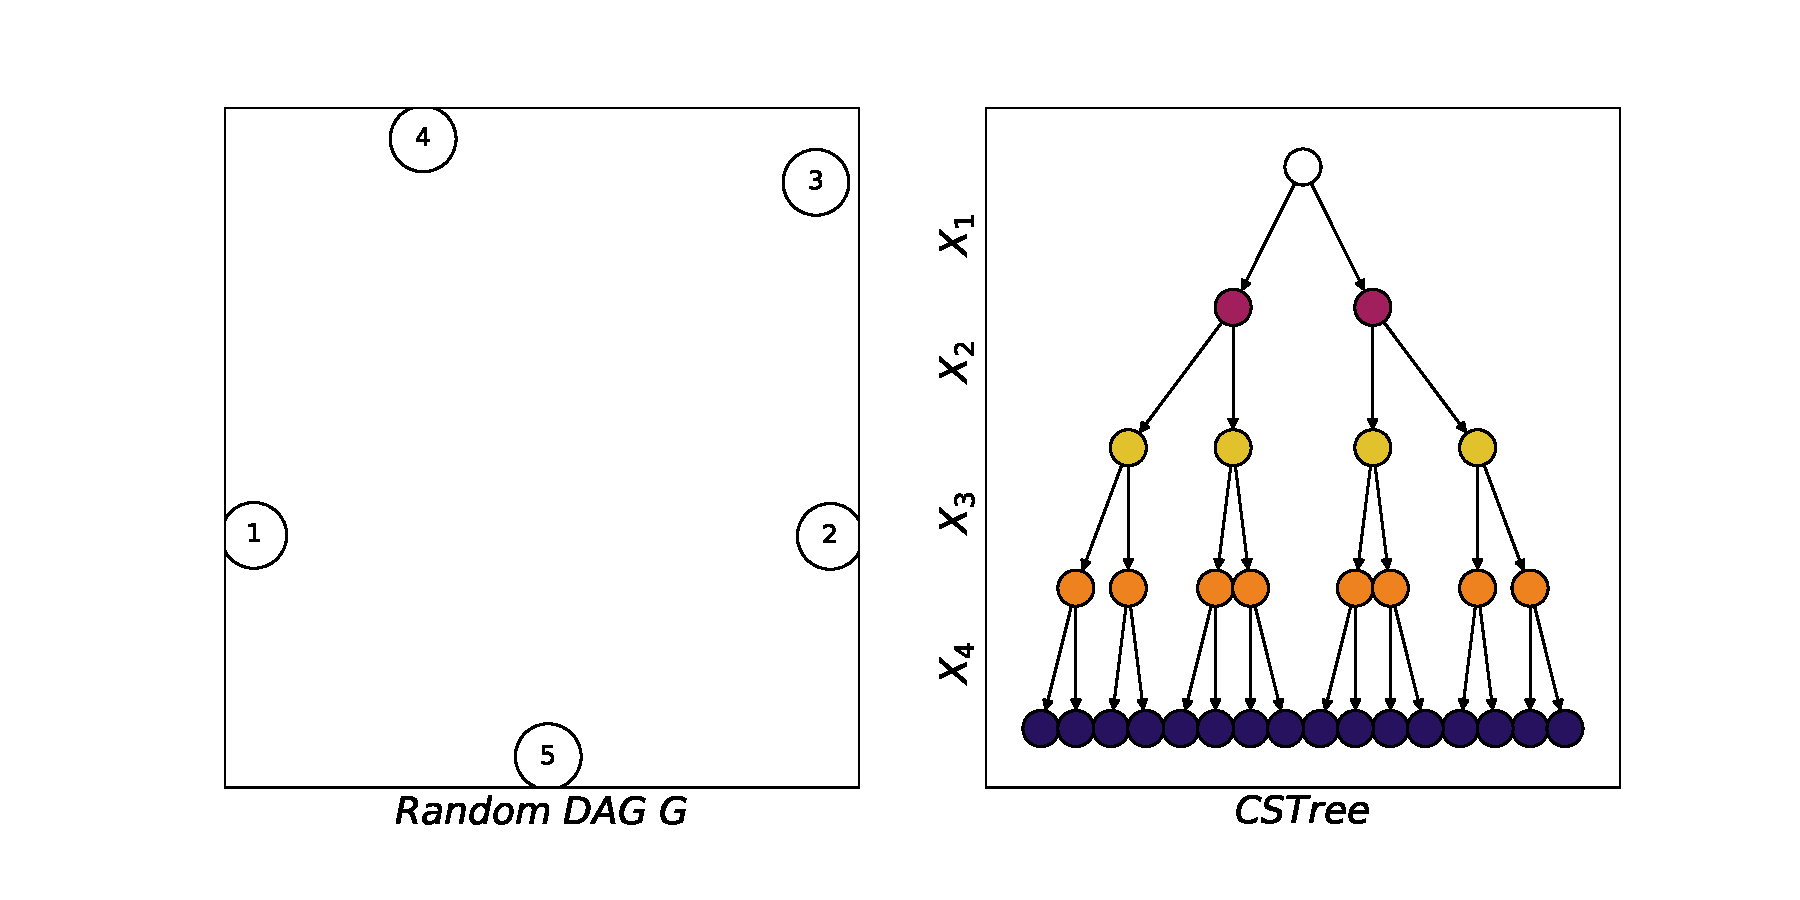
\includegraphics[width=1\linewidth]{figures/emptydagtocstree.pdf}}%
\caption{Generating the CSTrees for DAG with no edges using the ordering 1234 with Algorithm \ref{alg:dagtocstree}}
        
   \end{floatrow}
\end{figure}

The results are as expected since there are no conditional independence stations encoded in the fully connected, and no context specific independence statements since they are unable to encode them, meaning no 2 nodes share a fixed context and all stages have a single element. For the DAG with no edges, each variable is independent of each other, and each node has no parents thus by Proposition \ref{prop:dagandcstrees}

\section{Recovering the empty context DAG}
\label{sec:org789905a}
We start by generating random DAGs and generating the CSTrees as per Algorithm \ref{alg:dagtocstree}. This is done by first choosing the number of variables (nodes in the DAG) \(p\), and then choosing an edge with probability \(p_{edge} \in (0,1)\), and then keeping edge \((u,v)\) if and only if \(u<v\). We show the generated CSTree below, and recover the original DAG as a minimal context DAG with the empty context with Algorithm \ref{alg:mcdags}.

\begin{figure}[!h]\label{fig:dagtocstree_cstree}
   \begin{floatrow}
\ffigbox{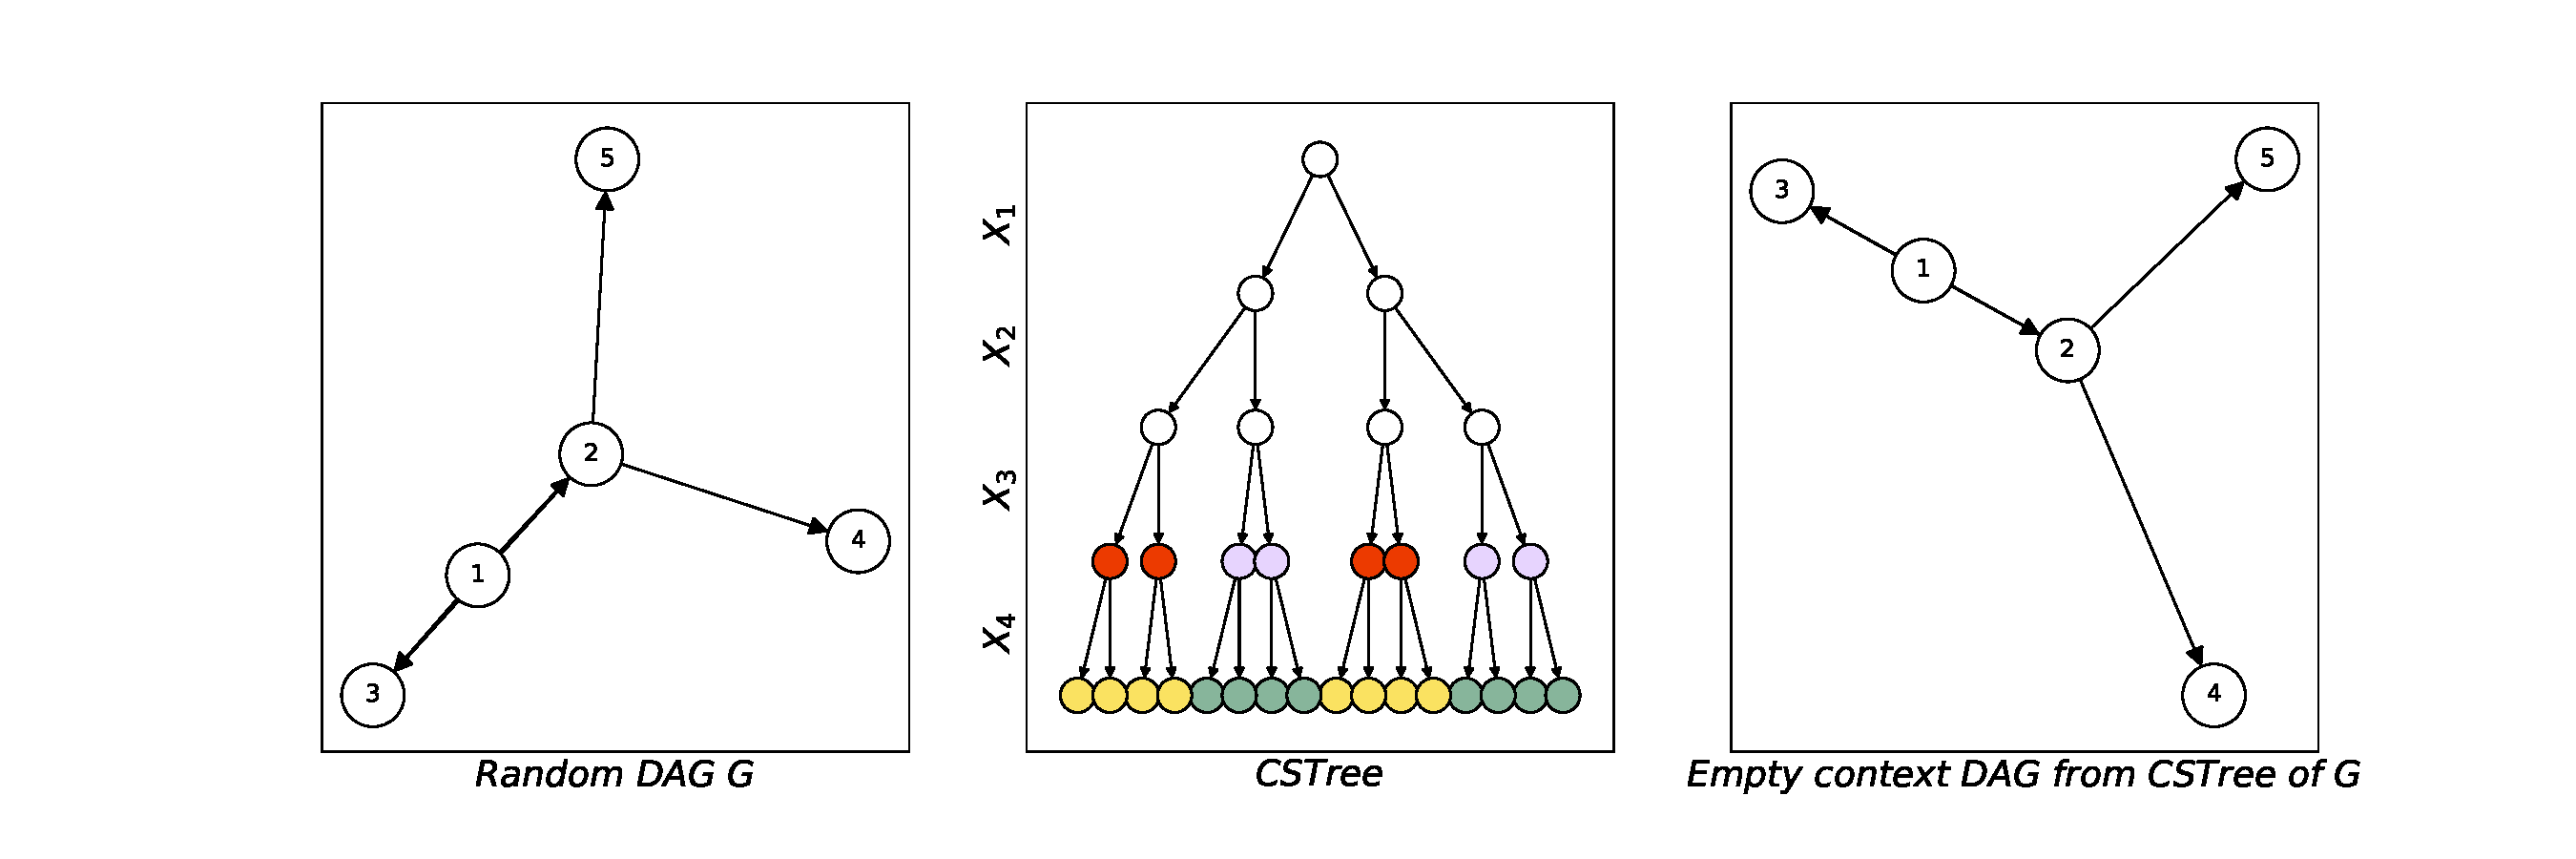
\includegraphics[width=1.1\linewidth]{figures/dagtocstreetoemptycontextdag.pdf}}%
\caption{Generating CSTrees from random DAGs and recovering the original random DAG from the CSTree with ordering 1234 using Algorithm \ref{alg:mcdags}}
        
   \end{floatrow}
\end{figure}


The following table summarizes the empirical space time complexity of generating a CSTree from certain random DAGs generated from the aforementioned procedure.

\begin{table}[htbp]
\caption{Statistics from generating CSTrees for random DAGs, Space refers to the amount of RAM occuppied by the CSTree structure, and time refers to the amount of time taken to encode the CI relations in the DAG to the CSTree.}
\centering
\begin{tabular}{r|r|r|r}
\hline
\(p_{edge}\) & DAG Nodes & Space  (GB) & Time  (s)\\
\hline
0.2 & 20 & 1.203 & 14\\
\hline
0.2 & 21 & 2.422 & 43\\
\hline
0.2 & 22 & 4.875 & 74\\
\hline
0.2 & 23 & 9.812 & 240\\
\hline
\end{tabular}
\end{table}

\section{Synthetic data}
\label{sec:orgb01549b}
Next we generate a random DAG \(\mathbb{G}\) using the procedure above, and then generate samples from this DAG, where each variable is binary valued. We then discard the DAG and apply Algorithm \ref{alg:cstreepc} on the generated samples. For nodes with edges, we sample the data by constructing a conditional probability distribution table by taking the parents of the nodes, and creating one row for each possible outcome of the parents. In this binary case, if a variable \(X_i\) has \(d\) parents \(X_{PA_{X_1}},...,X_{PA_{X_d}}\), the corresponding table has \(2^d\) rows. The 2 columns represent the outcome 0 and 1 respectively. The probability values are filled by taking a row corresponding to some outcome of the parents, and assigining the probability of \(X_i=0\) under this outcome to be distributed uniformly between \([0.01,0.2]\) or \([0.8,0.99]\) each with a probability 0.5. The probability for \(X_i=1\) under this outcome is then simply computed such that the probabilities sum to 1. For the variables corresponding to nodes with no edges, we give them a Bernoulli distribution with a parameter chosen uniformly between \([0,1]\) for each such variable.



We start by generating 100000 samples on 4 binary variables using the above procedure and learning the CSTree and recovering the minimal context DAGs. We show the results below.
\begin{figure}[!h]\label{fig:synthetic_exp1}
   \begin{floatrow}
\ffigbox{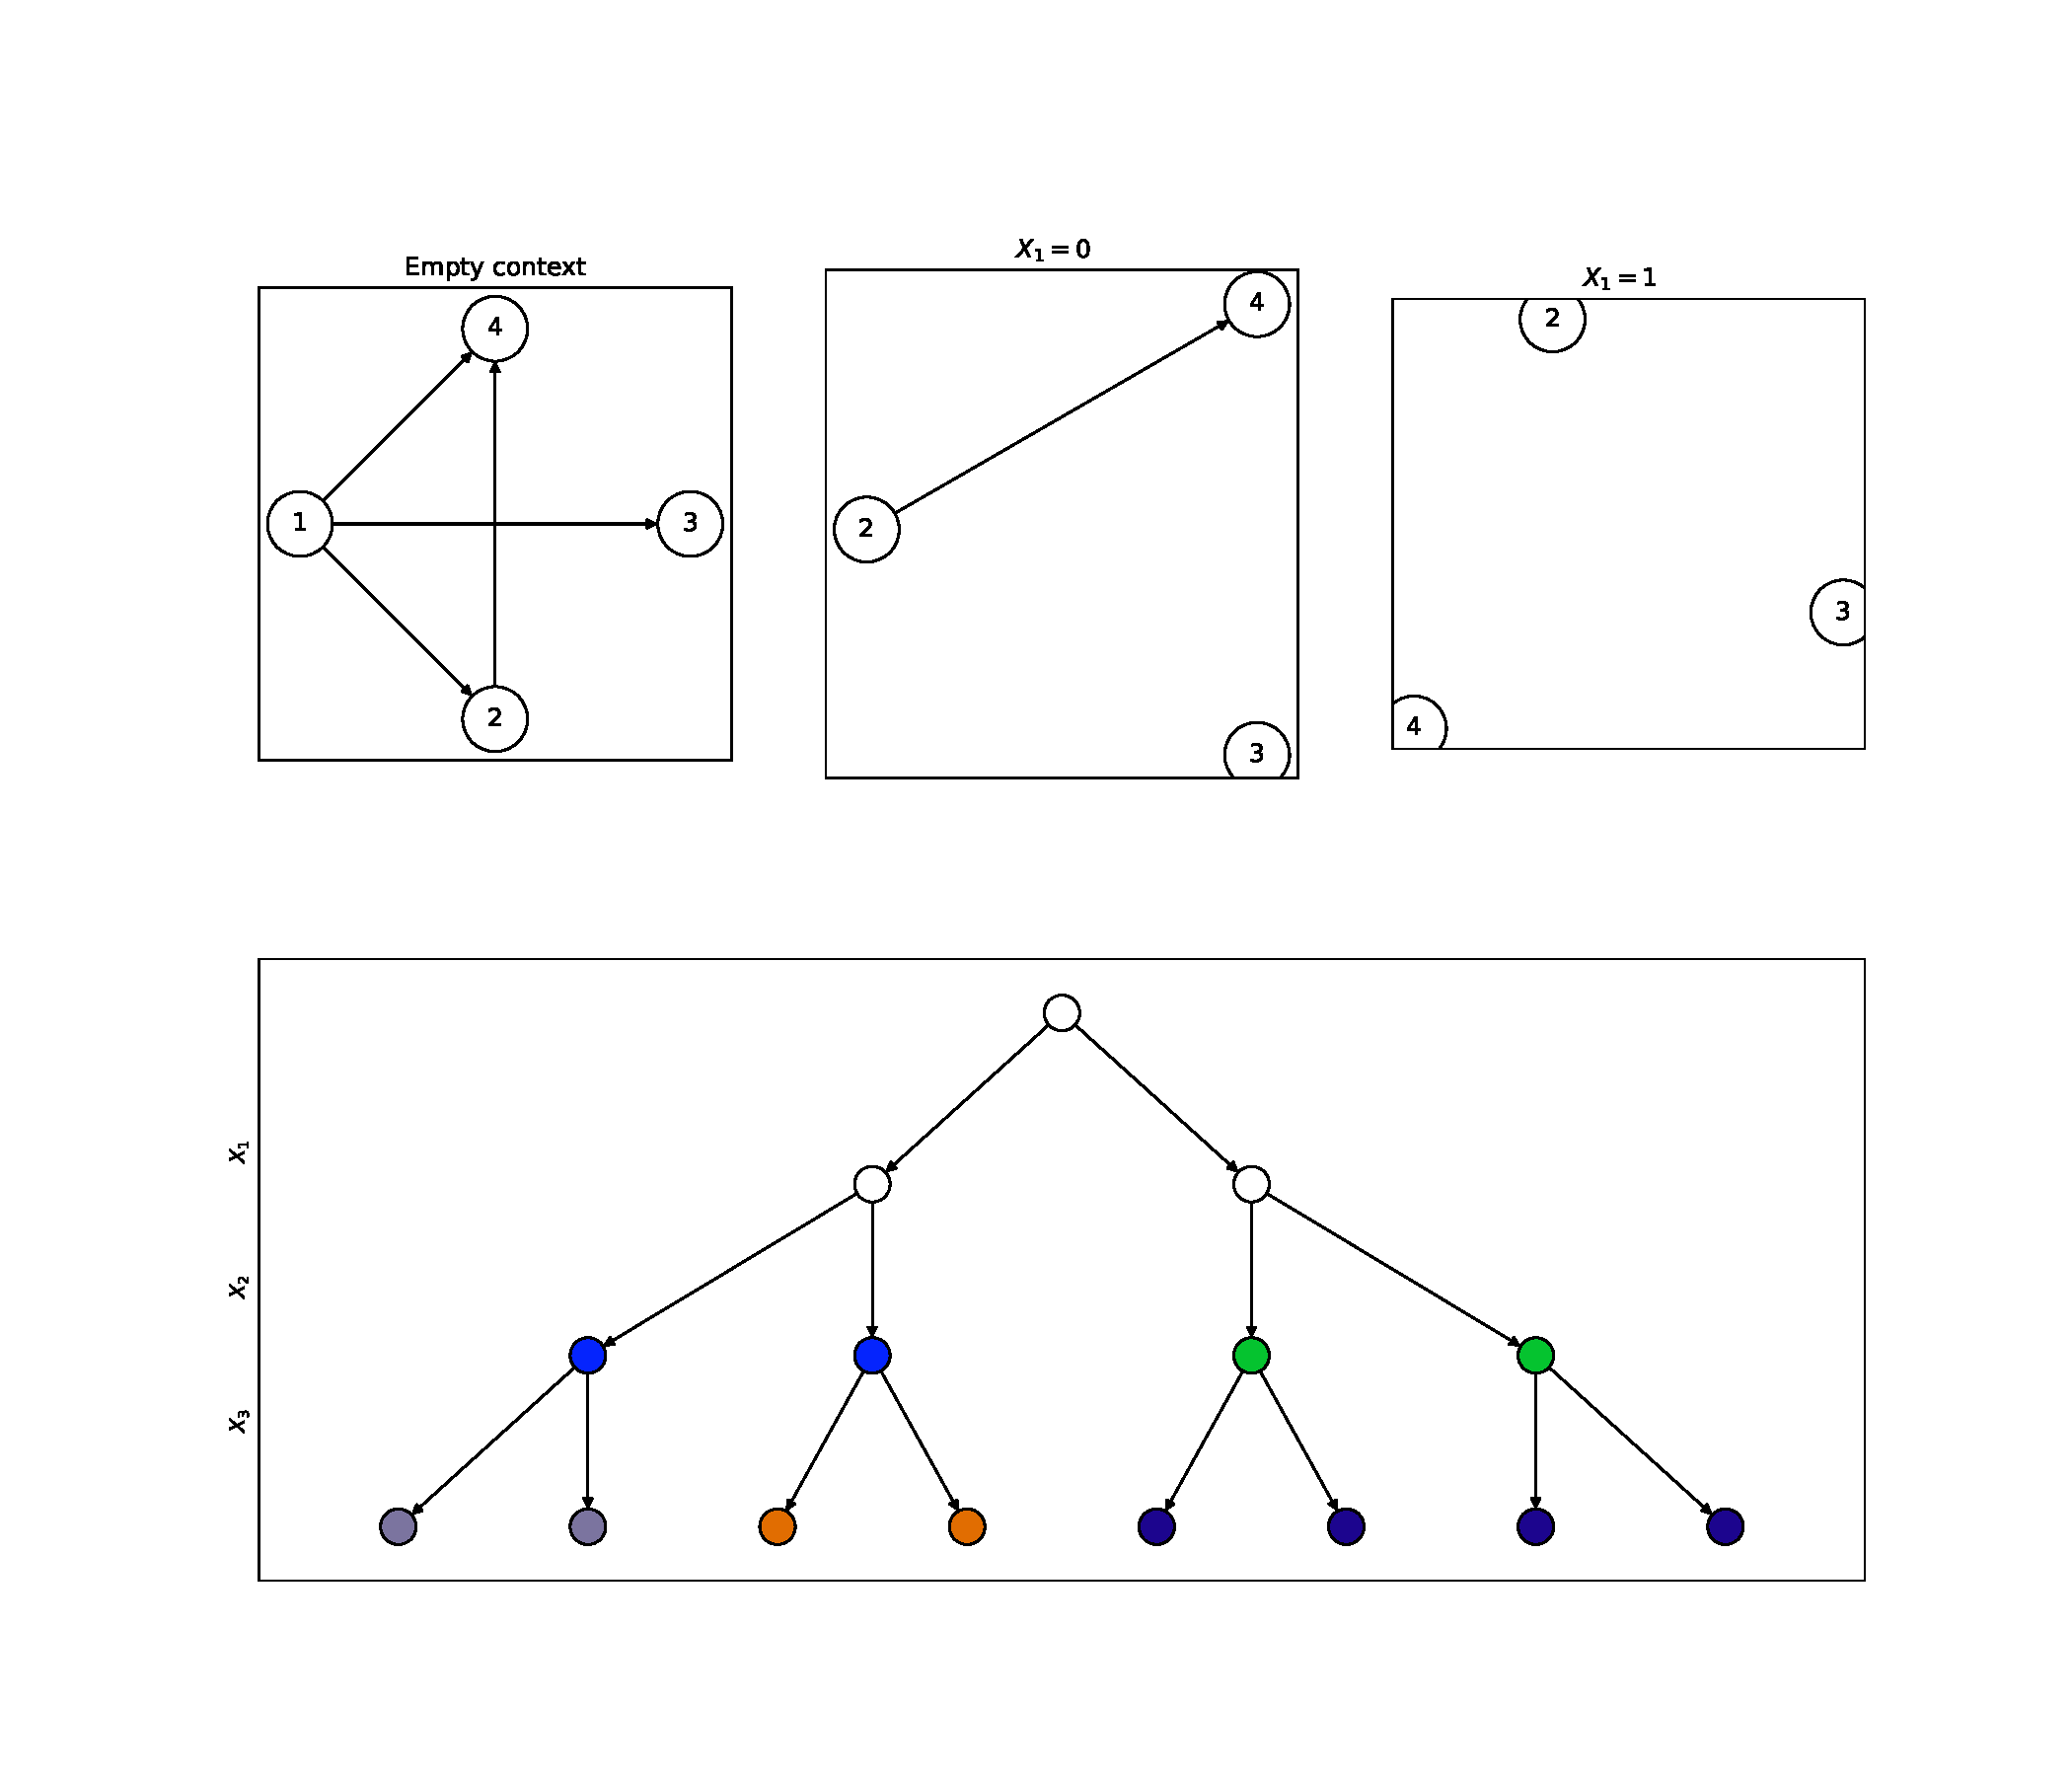
\includegraphics[width=1.1\linewidth]{temp/eppswdagnotremovingskewed.pdf}}%
\caption{Generating CSTrees from datasets generated by random DAGs and learning the context specific causal structure using Algorithm \ref{alg:cstreepc} and \ref{alg:mcdags}}
        
   \end{floatrow}
\end{figure}




In order to assess the influence of the CI relations from the DAG in the final CSTree, we tested the use of Algorithm \ref{alg:cstreepc} with the following experiment. First we generate a dataset from the above procedure, then we run Algorithm \ref{alg:cstreepc} on this dataset with and without using the CI relations from the CPDAG learnt in the first step. Below is an example where the DAG picks up a conditional independence relation which is not picked up by strictly running only the context specific independence tests.


\begin{figure}[H]\label{fig:synthetic_exp2a}
   \begin{floatrow}
\ffigbox{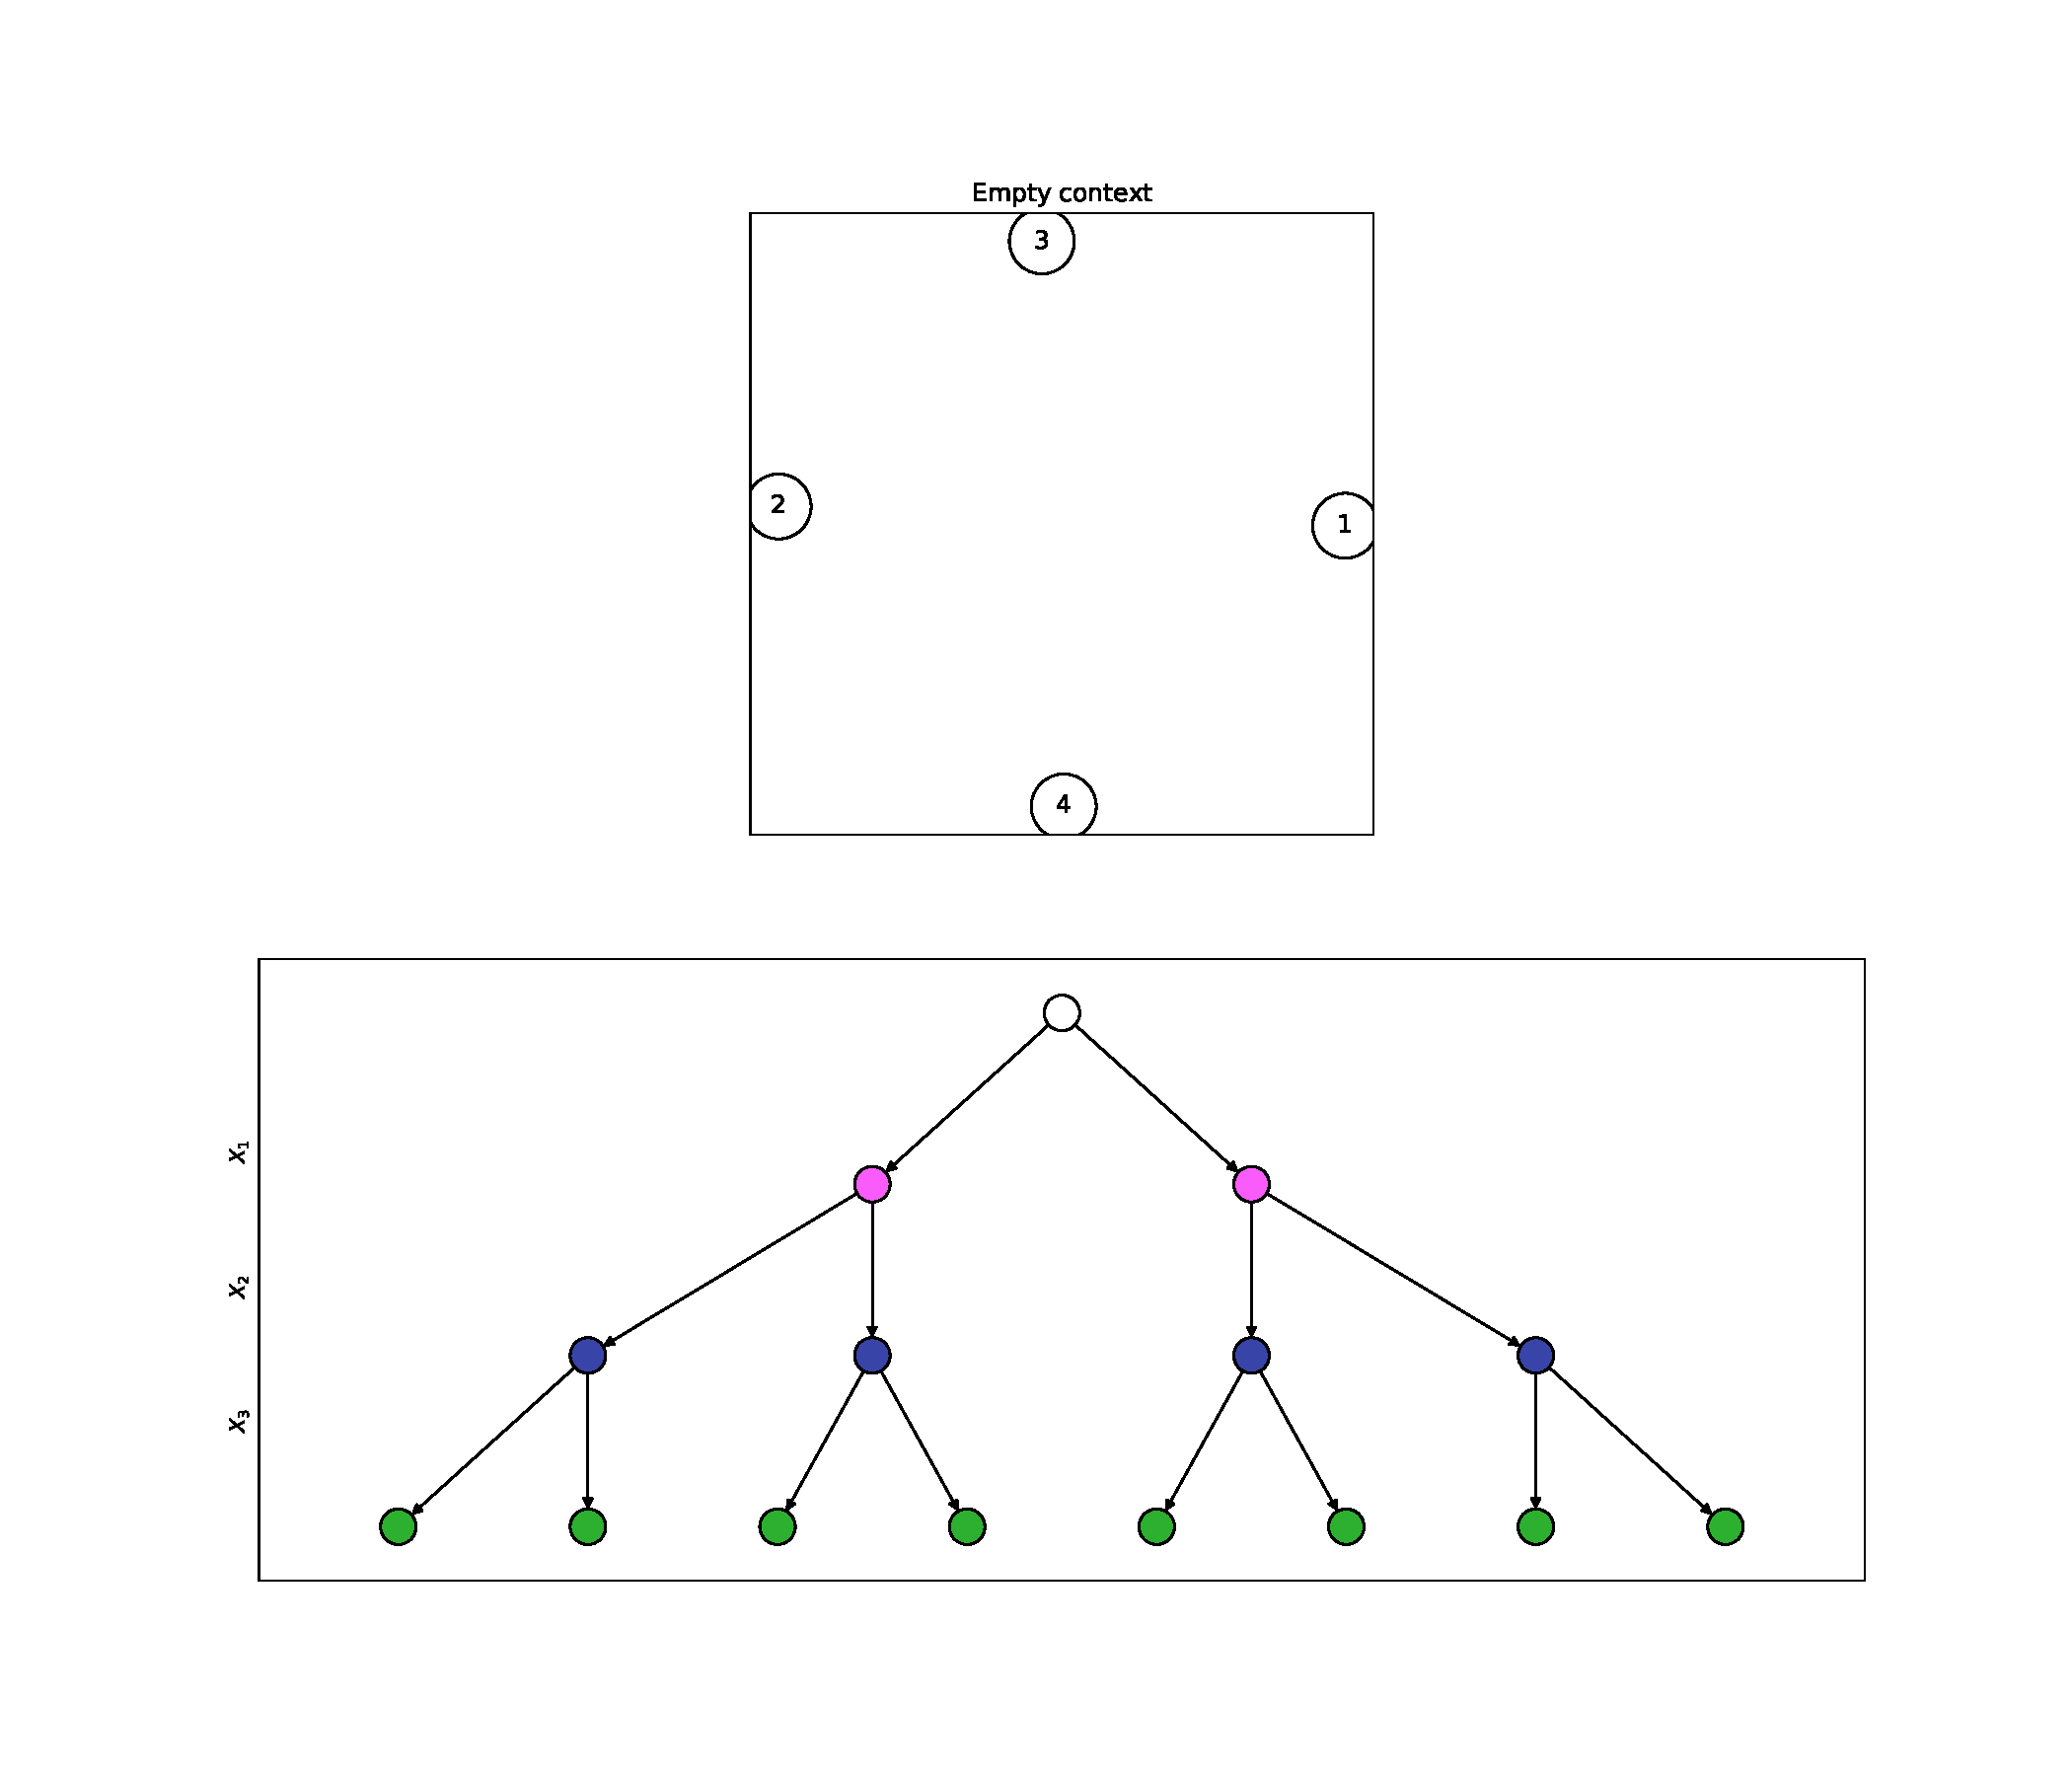
\includegraphics[width=1.1\linewidth]{temp/andersonwdag_subsample.pdf}}%
\caption{CSTree learnt using the CI relations from the DAG, which encodes the relation $X_3 \indep X_2,X_1$}
        
   \end{floatrow}
\end{figure}
\begin{figure}[H]\label{fig:synthetic_exp2b}
   \begin{floatrow}
\ffigbox{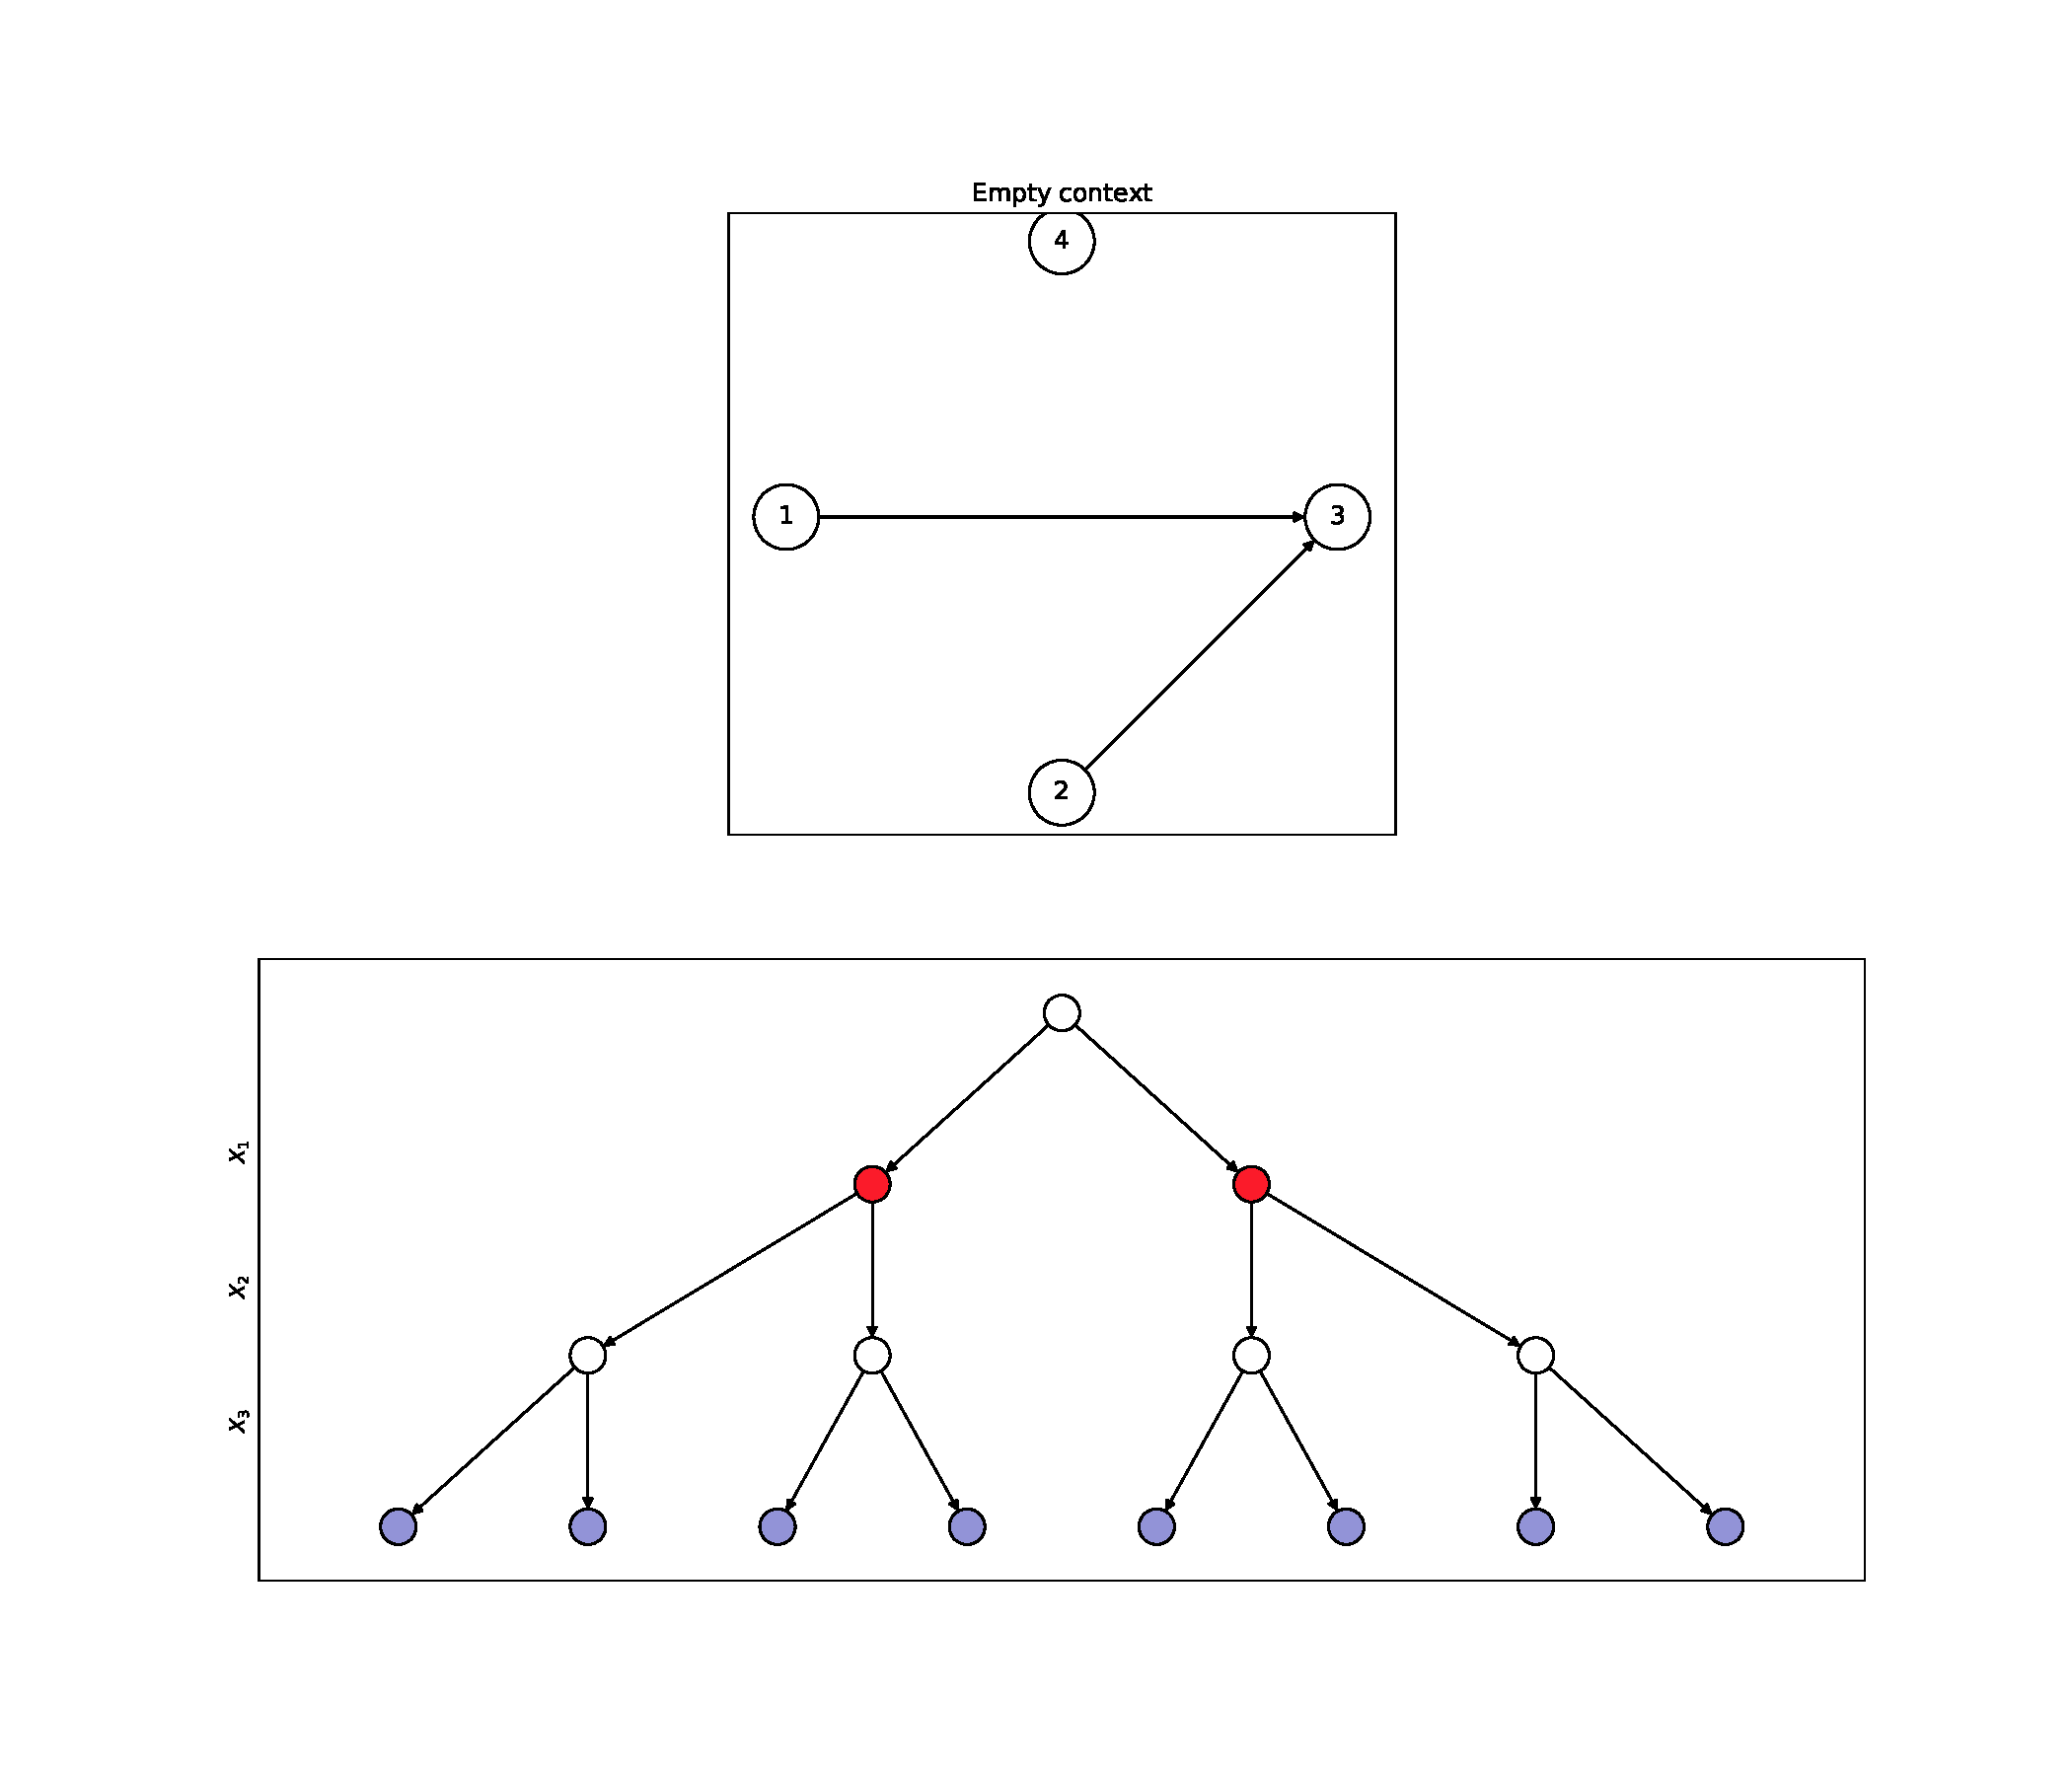
\includegraphics[width=1.1\linewidth]{temp/andersonwoutdag_subsample.pdf}}%
\caption{CSTree learnt without the CI relations from the DAG, which does not encode the relation $X_3 \indep X_2,X_1$ unlike when using the DAG on the same dataset}}
        
   \end{floatrow}
\end{figure}


\section{Coronary disease data}
\label{sec:org703301b}

This is a dataset consisting of features which might increase the risk for coronary thrombosis, and consists of 1841 samples from men \cite{reinis-1981-progn-signif}. These features are detailed below.
\begin{center}
\begin{tabular}{ll}
\hline
Variable & Outcome space\\
\hline
Smoking & \{Yes,No\}\\
Strenuous mental work & \{Yes,No\}\\
Strenuous physical work & \{Yes,No\}\\
Systolic blood pressure & \{<140,>140\}\\
Ratio of beta and alpha lipoproteins & \{<3,>3\}\\
Family history of coronary heart disease & \{Negative,Positive\}\\
 & \\
\end{tabular}
\end{center}
This data set does not require further pre-processing since the outcome space is already categorical, and there were no missing values.




\begin{figure}[!h]\label{fig:coronary1}
   \begin{floatrow}
\ffigbox{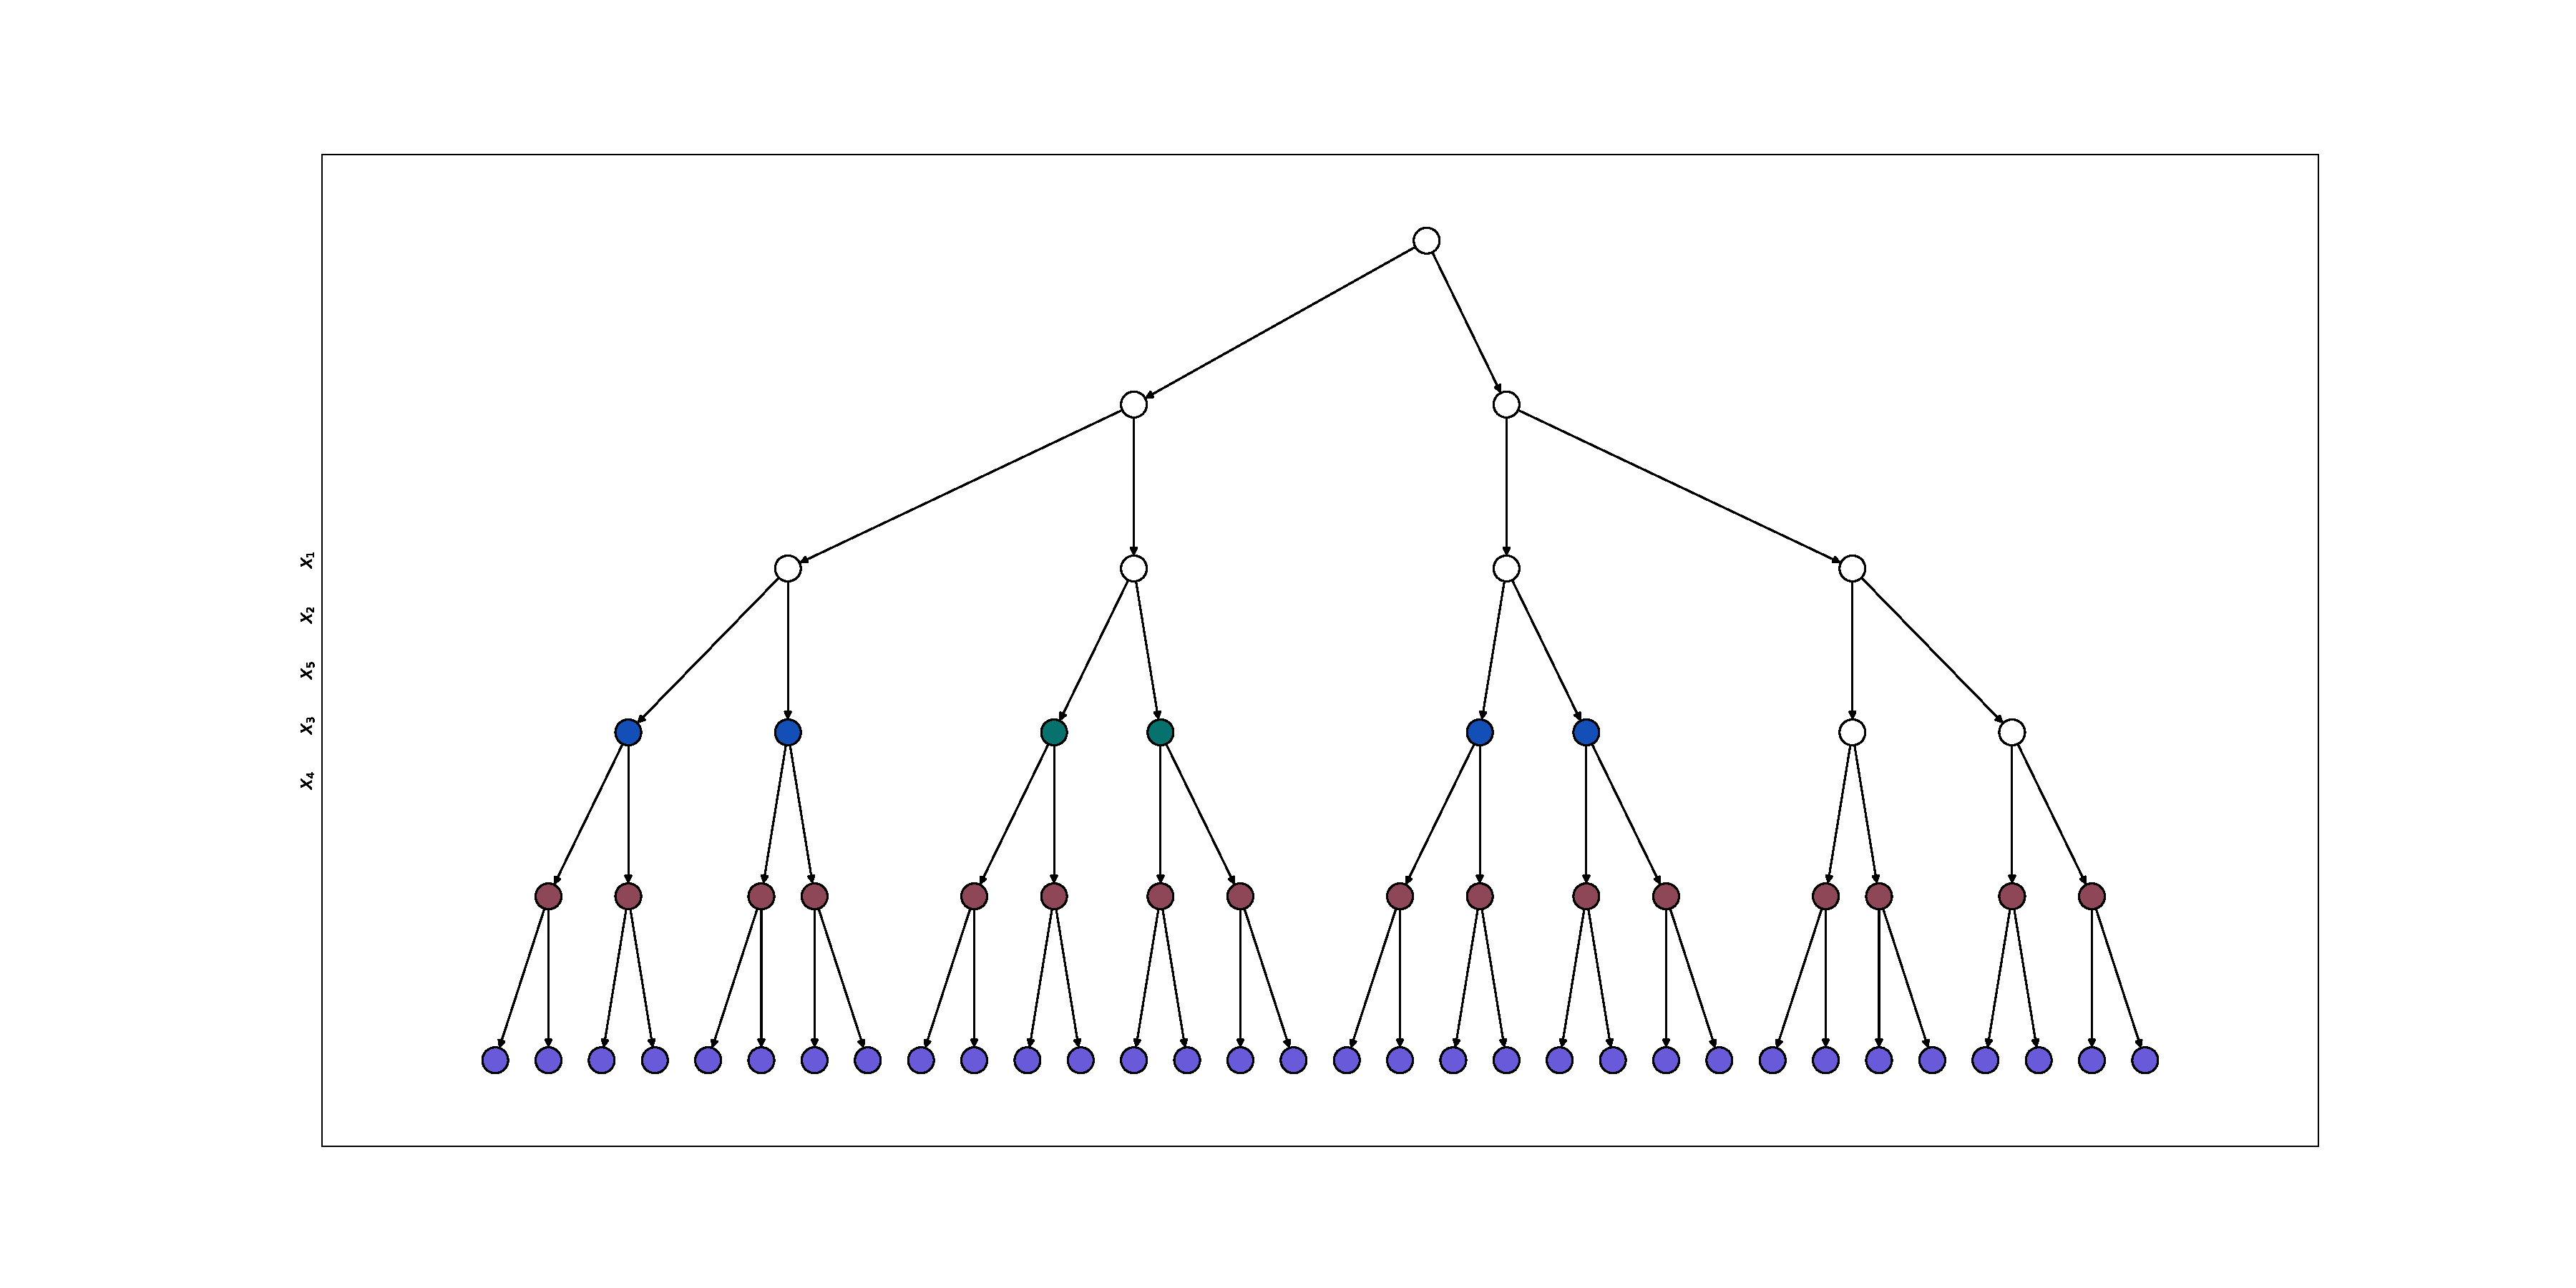
\includegraphics[width=1.1\linewidth]{temp/coronary_nonindep.pdf}}%
\caption{Example of CSTree learnt on the coronary dataset which was not the independence model which has the ordering 125346}
        
   \end{floatrow}
\end{figure}


\section{Mice protein expression data}
\label{sec:orgf88f513}
This is a dataset with expression levels of 77 proteins, measured in the cerebral cortex of 8 classes of mice \cite{higuera-2015-self-organ}. There are 38 control mice and 34 trisomic mice, and for each of them 15 separate measurements were taken which gives a total of 1080 samples. The aim is to identify features that can discriminate between the 8 classes that make up all possible combinations of the following 3 binary features - Control or Trisonomy, stimulated to learn or not, injected with saline or memantine. This dataset had missing values, which is why we handle by first inspecting the missing value counts for each feature and then removing features which had had 180 or more missing values. This removes the expression data corresponding to the columns \(BAD_N, BCL2_N, H3AcK18_N, EGR1_N, H3MeK4_N\). This still leaves 72 features, which we further reduce by recursive feature elimination \cite{guyon-2002} where we first train a linear support vector classifier on all the features and prune the least important features in a greedy manner until we arrive at the number of features we want, which in this experiment we set as 6. After this we compute the medians for each feature and assign each feature to take binary outcomes depending on whether or not the value is above or below the median. With the predictor class, which takes 8 possible values, this is a system with 7 variables. We choose this number mainly because the amount of samples drastically reduce as we fix contexts when we go down each level.


Applying Algorithm \ref{alg:cstreepc} on this dataset resulted in 108 CSTrees with the minimum number of stages, which is 518. Excluding the singleton stages arising from the last level, this is 6 stages, which are once again extremely sparse.


Running the algorithm without using the CI relations from the DAG however can result in a more complex CSTree model for example the one given below for the causal ordering 1275634.

\begin{figure}[!h]\label{fig:mice1}
   \begin{floatrow}
\ffigbox{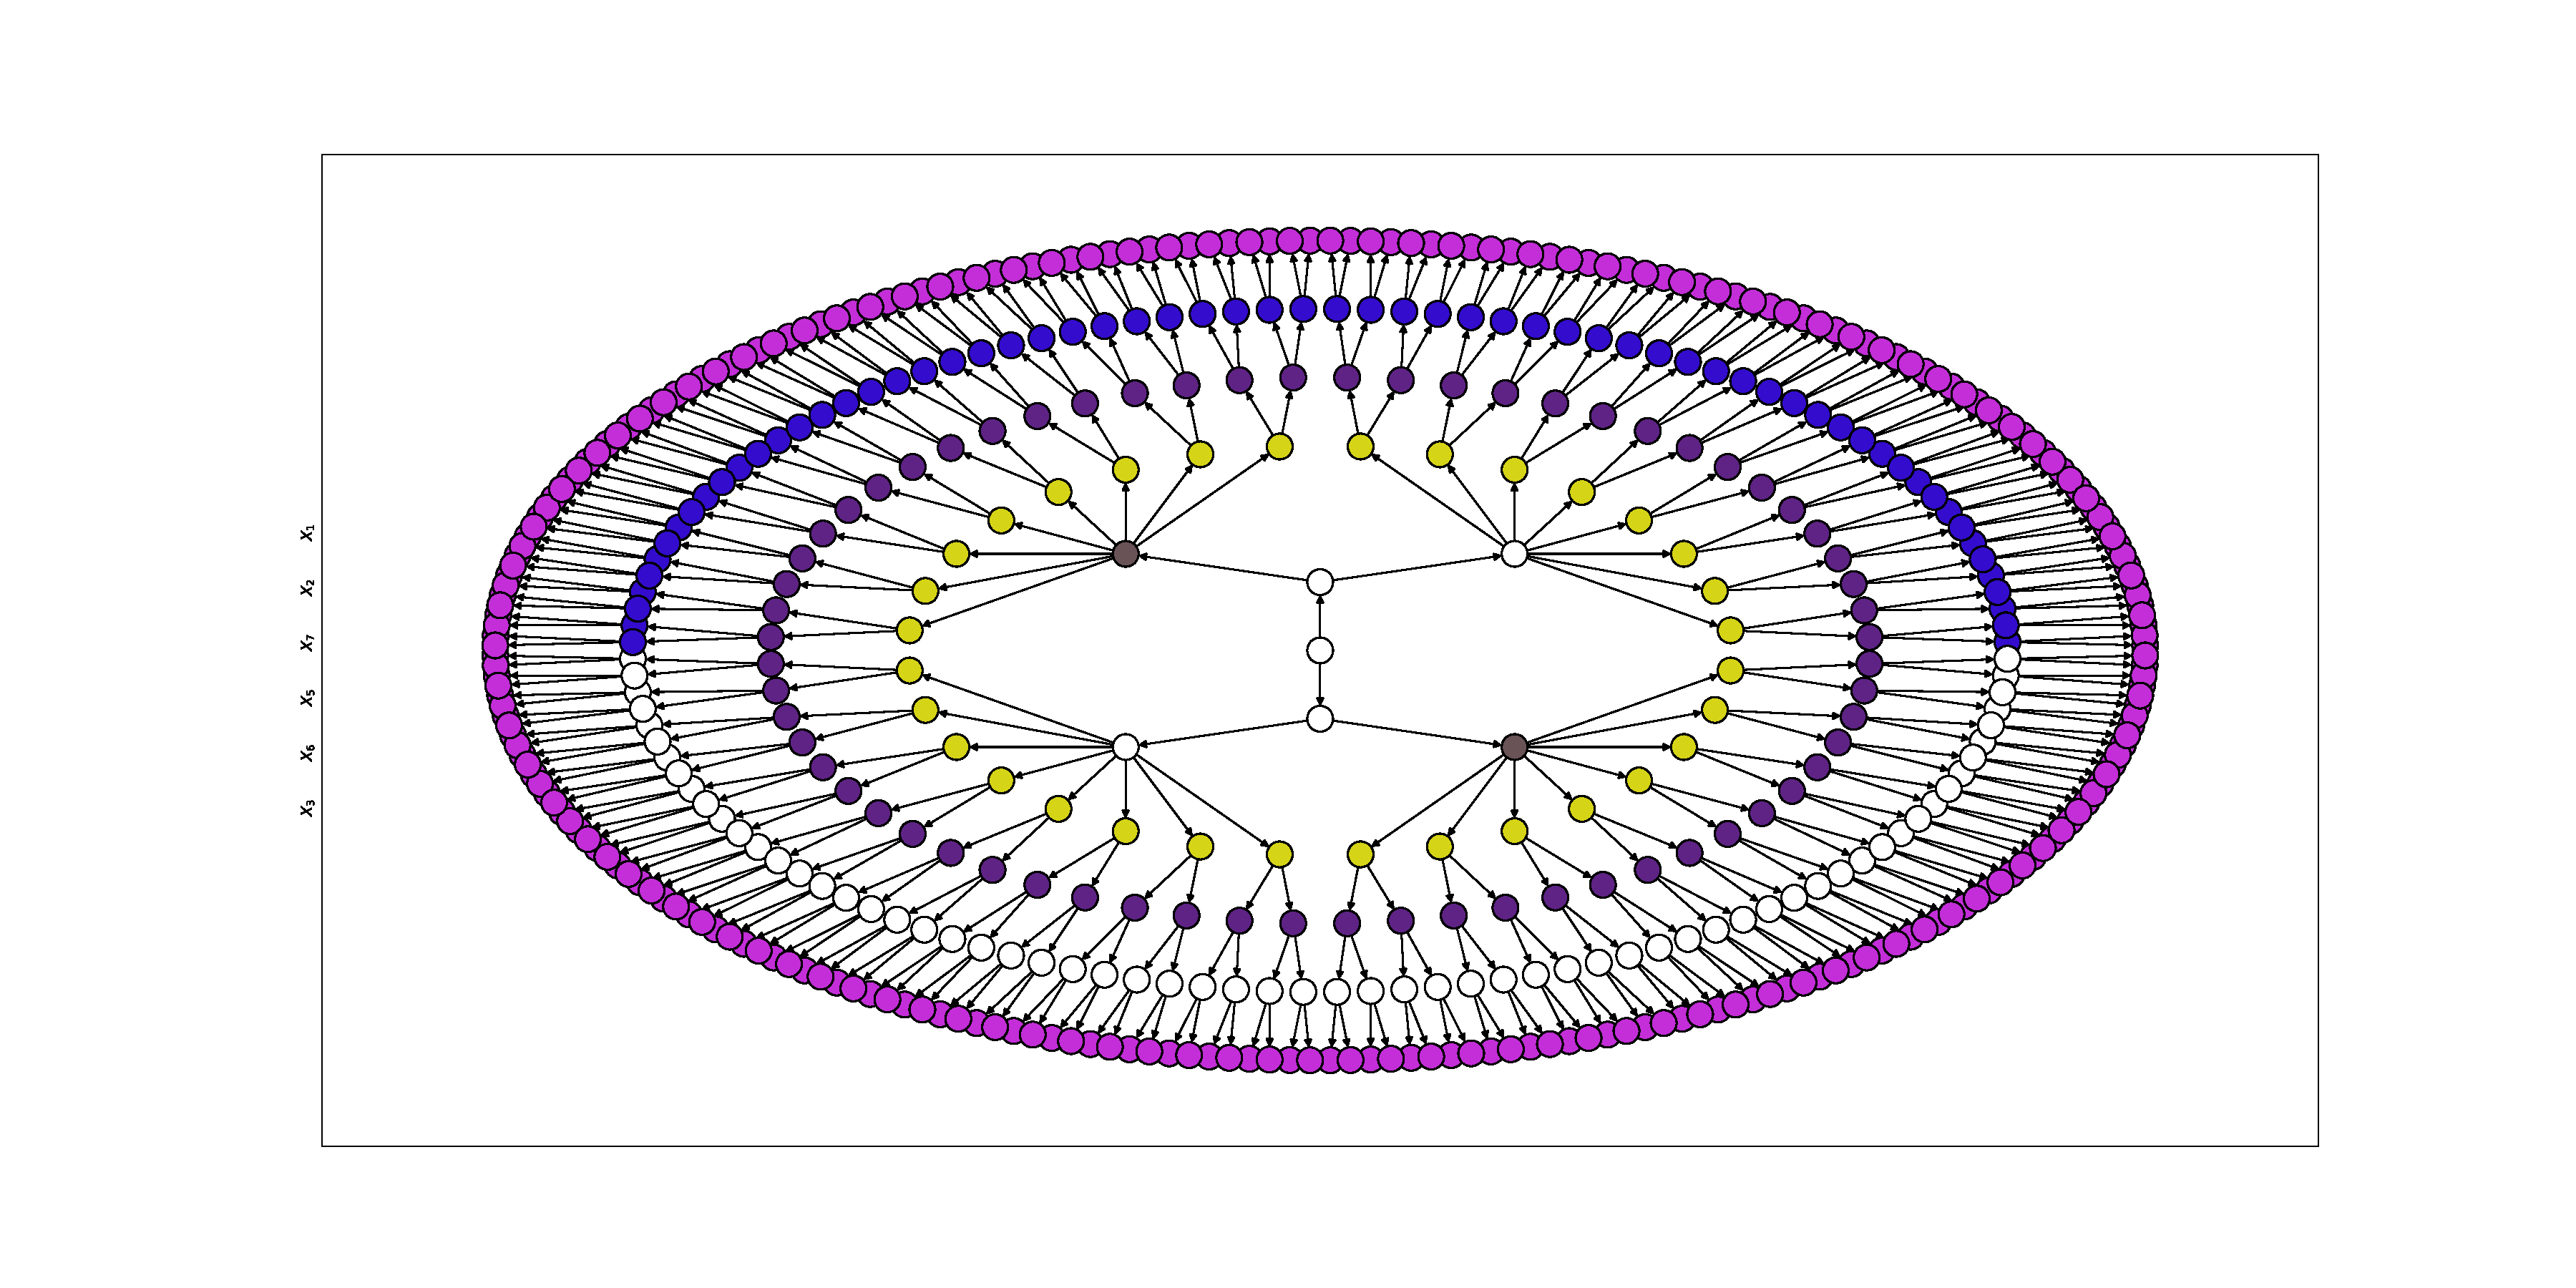
\includegraphics[width=1.1\linewidth]{temp/mice6_nodag1_cstree.pdf}}%
\caption{CSTree with ordering 1275634 learnt from the mice cortex data.}
        
   \end{floatrow}
\end{figure}


It is important to note that many context specific independence tests are skipped due to fewer data.



\section{Supersymmetry data}
\label{sec:org481fe88}

This is a simulated dataset involving 8 kinematic features measured by detectors in a particle accelerator alongside 10 more high-level features which are functions of the original 8 features \cite{baldi-2014-searc-exotic}. The aim is is to identify the class label for each sample which denotes whether the measurement corresponds to a signal or background event. The dataset contains in total 5000000 samples. There are no missing values in this dataset, and we apply it on the 8 low-level features, and after taking a random subsample of size 100000. Due to the high number of possible causal orderings, we show below the first CSTree learnt.

\begin{figure}[!h]\label{fig:susy1}
   \begin{floatrow}
\ffigbox{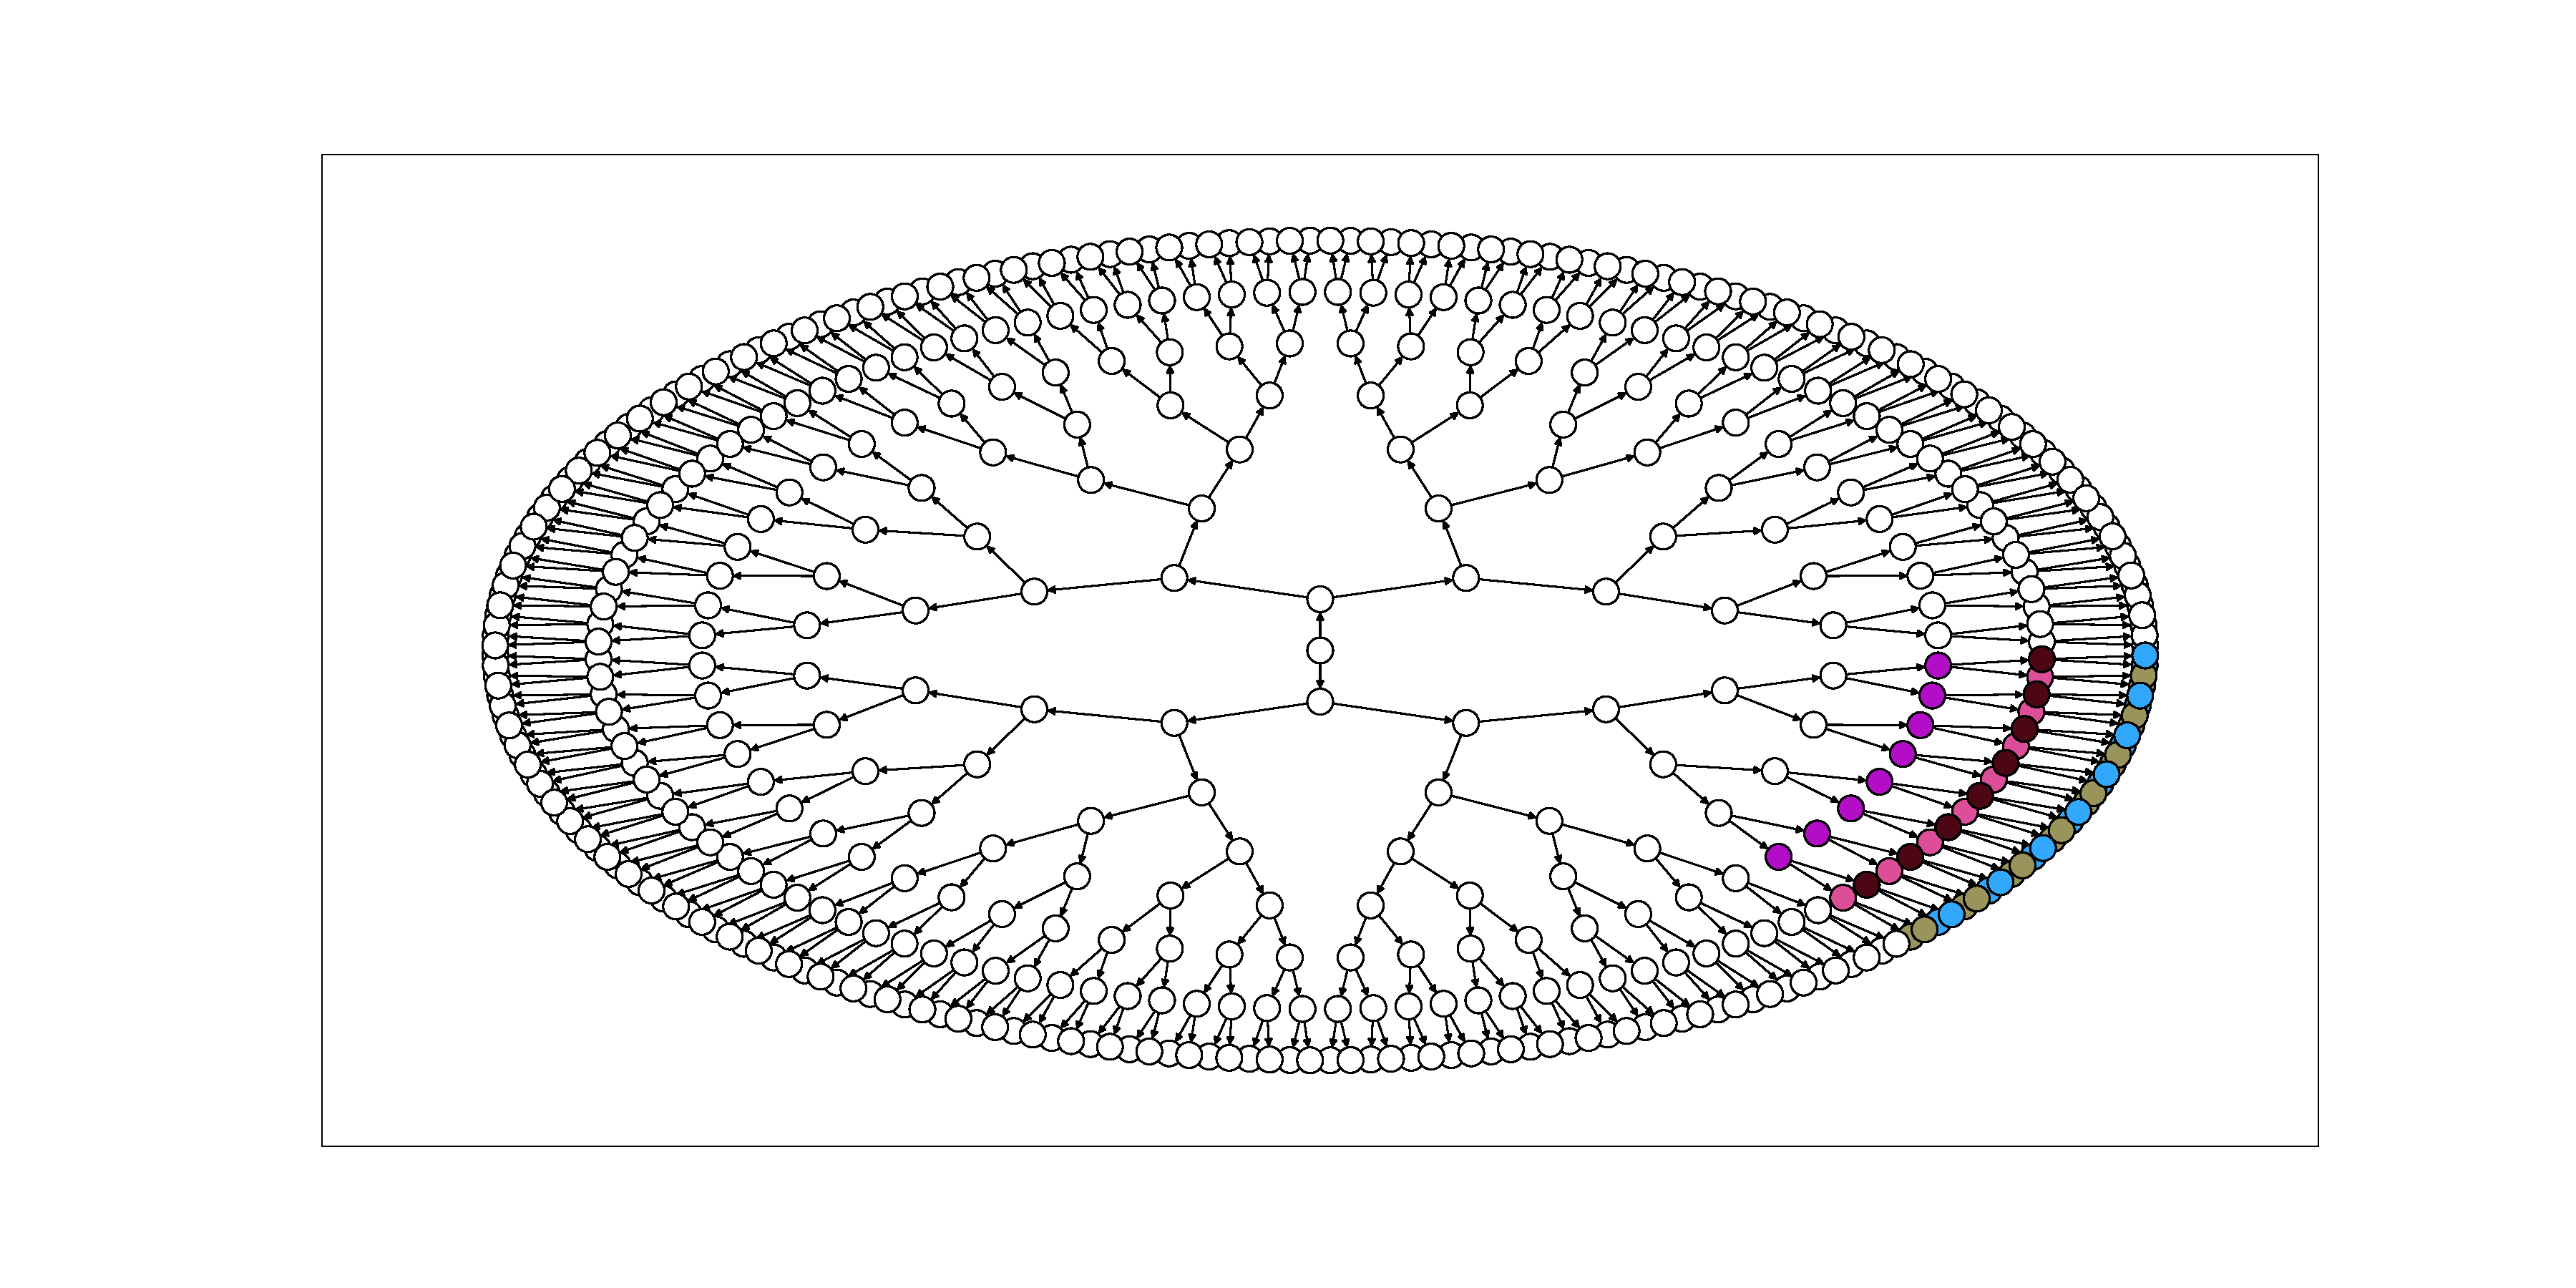
\includegraphics[width=1.1\linewidth]{temp/susy1_cstree.pdf}}%
\caption{First CSTree learnt from the supersymmetry dataset.}
        
   \end{floatrow}
\end{figure}

It is expected that since the supersymmetry data involves many causal interactions, there will be few independence relations, which is what we see from the CSTree.


\section{Discussion of empirical performance}
\label{sec:org3b01116}

In practice, the rapidly decreasing amount of samples as we go to the later levels of the CSTree results in skipped tests. This is in part due to the implementation of the statistical tests not taking samples less than 5, or not taking samples consisting of a single outcome. In terms of context specific conditional independence testing, we use the Epps and Singleton test \cite{epps-1986-omnib-test} and the Anderson-Darling test \cite{scholz-1987-k-sampl}, both of which are implementing in scipy \cite{virtanen-2020-scipy}. We observe that there are no significant differences between these tests. Due to the fact that many statistical tests are run on significantly imbalanced sample sizes, in the presence of small data it might be a good idea to perform the statistical test only if a certain criteria is met, for example, run the test only if both samples are atleast half of their mean. 


The instability of the CI testing from the PC algorithm step also plays a main role, for example in the synthetic DAG experiments, the order \(123\cdots p\) must always be a valid order however there are instances where no DAG derived from the CPDAG contains this as a valid ordering. This may also present itself to be a problem if we have partial knowledge of the ordering, for example in the mice cortex data experiment, it is plausible to think of the predictor class to be a function of the gene expression levels, however the CPDAG contains no DAG with an ordering such that this variable comes at the very last.


One important aspect of this process is to choose the best CSTree from all possible causal ordering, which is a model selection problem. In Algorithm \ref{alg:cstreepc} we opt to choose the one with the fewest stages since it relates to choosing the model with the fewest parameters, i.e. the simplest model. This goes in hand with the principle of Occam's razor - in the face of many possible models, choose the simplest model. Here a simple model refers to one which has few parameters. In practice however we see that problems arising due to misleading conditional independence tests and small data samples might lead to the simplest model being too simple, compromising the fit to the data.



\chapter{Conclusions}
\label{sec:orgba6578c}
\section{Summary}
\label{sec:org6671130}
We start with DAGs as a means to encode CI relations, and how one can use the characterization of Markov Equivalence in DAGs to learn causal structure through CI testing. We then cover the limitations of CI relations in comparison to CSI relations, and go over CSTrees as a means to encode such CSI relations. We then show how one can learn these CSI relations from observational data and learn a CSTree, and how to compute minimal contexts which are important when it comes to visualizing higher dimensional CSTrees. We then apply these techniques to synthetic and real data.


\section{Future work}
\label{sec:org6588be6}
One of the more natural extensions of this work is to learn CSTrees from interventional data. This can already be done with DAGs \cite{yang-2018-charac-learn}. On the topic of model selection, it might be interesting to see the applicability of Bayesian model selection for CSTrees, whereby the model evidence is used as the basis for comparing models which automatically penalizes over-complex models whilst also penalizing models which do not agree with the observed data \cite{mackay-1992-bayes-inter}. Similar approaches have been applied to Gaussian DAG models \cite{castelletti-2020-bayes-model}. Generalization to missing data problems would also be an interesting avenue, considering that the PC algorithm has been recently extended for missing data instances in DAGs \cite{tu-2019-causal-discov}. But perhaps the most impactful extension would be formulating the problem of finding the best CSTree into a continuous optimization problem, which can lead to scalable score based methods. Recent work has formulate the problem of searching for the best DAG according to some metric by using a characterization of acyclicity that is smooth and exact, allowing the conversion of the combinatorial problem into a purely continuous problem \cite{zheng-2018-dags-no-tears}.  






 \newpage 



\bibliographystyle{unsrt}
\bibliography{../../../Dropbox/org/bibliography/references}

 \newpage 

\chapter{Appendix A}
\label{sec:orgaa99d5f}
\section{Remarks on implementation}
\label{sec:org60d9014}
Implementation of this work was done in Python. Draft code repository is available at github.com/mnazaal/masters-thesis. This document was generated with org-mode. Use of scikit, pandas, numpy. Test driven development with pytest.
\end{document}